\chapter{Applications}
\label{chapt:apps}
\index{Applications}
\index{MARF!Applications}

$Revision: 1.18 $

This chapter describes the applications that employ {\marf}
for one purpose or another. Most of them are our own applications
that demonstrate how to use various {\marf}'s features. Others
are either research or internal projects of their own. If you
use {\marf} or its derivative in your application and would like
to be listed here, please let us know at \url{marf-devel@sf.lists.net}.


%
% Internal Research Applications
%

\section{MARF Research Applications}
\index{MARF!Research Applications}

%
% SpeakerIdentApp
%

\subsection{SpeakerIdentApp - Text-Independent Speaker Identification Application}
\index{Applications!SpeakerIdentApp}
\index{Research Applications!SpeakerIdentApp}

\api{SpeakerIdentApp} is an application for text-independent
speaker identification that exercises the most of the {\marf}'s
features.
\api{SpeakerIdentApp} is broadly presented through
the rest of this manual.


%
% ZipfLawApp
%

\subsection{Zipf's Law Application}
\index{Zipf's Law}
\index{Zipf's Law!Application}
\index{Applications!Zipf's Law}

$Revision: 1.15 $

Originally written on February 7, 2003.

\paragraph{The Program}

%is Java has built-in \api{StreamTokenizer}; you just have
%to instruct it how you want tokens to look like, and get
%them from any input stream, one-by-one. Java also provides
%us with built-in types and data-structures to manage
%collections (build, sort, store/retrieve) efficiently.

\paragraph{Data Structures}

The main statistics ``place-holder'' is a \api{oStats} \api{Hashtable}, nicely
provided by {\java}, which hashes by words as keys to other
data structures, called \api{WordStats}. The \api{WordStats} data structure
contains word's spelling, called lexeme (borrowed this term
from compiler design), word's frequency (initially $0$), and
word's rank (initially $-1$, i.e. unset). \api{WordStats} provides a typical
variety of methods to access and alter any of those three values.
There is an array, called \api{oSortedStatRefs}, which will eventually
hold references to \api{WordStats} objects in the \api{oStats} hashtable in
the sorted by the frequency.

Hashtable entry might look like this in pseudo-notation:

\verb+{ <word> } -> [ WordStats{ <word>, <f>, <r> } ]+

\subsubsection{Mini User Manual}

\paragraph{System Requirements}

The program was mostly developed under Linux, so there's
a \file{Makefile} and a testing shell script to simplify some routine tasks.
For JVM, any JDK 1.4.* and above will do. \tool{bash} would be nice
to have to be able to run the batch script. Since the application
itself is written in {\java}, it's not bound to specific architecture,
thus may be compiled and run without the makefiles and scripts
on virtually any operating system.

\paragraph{How To Run It}

There are at least three ways how to run the program, listed in order of complexity
(in terms of number of learning and typing involved).
In order for the below to work you'd need some corpora in
the same directory as the application.

\paragraph{Using the \tool{testing.sh} Script}

The script is written using \tool{bash} syntax; hence, \tool{bash} should be
present. The script ensures
that the program was compiled first, by invoking \tool{make}, then
in a for loop feeds all the \file{*.txt} files (presumably our corpora) along with the \file{ZipfLaw.java}
program itself to the executable, one by one, and redirects its standard output
to the files as \file{$<$corpus-name$>$[$<$options>$]$.log} in the current directory. These files will contain the
grouping of the 100 most frequent words every 1000 words as well as frequency-of-frequency counts at the end.

\noindent
Type:

\verb+./testing.sh+

\noindent
to run the batch through with the default settings.

\verb+./testing.sh <options>+

\noindent
to override the default settings with $<$options$>$. $<$options$>$ are the same
as that of the \api{ZipfLaw} application (see \ref{sect:zipf-law-app}).

\paragraph{Using \file{Makefile}}

If you want to build and to run the application just for individual,
pre-set corpora, use the \tool{make} utility provided with UNIXen.

Type (assuming GNU-style \tool{make}, or \tool{gmake}):

\noindent
\verb+make+

	to just compile the thing

\noindent
\verb+make <corpus-name> [ > <filename>.log ]+

	to (possibly compile if not done yet) and run it for the corpus
	\verb+<corpus-name>+ and to optionally redirect output to the file
	named \verb+<filename>.log+
	The \verb+<corpus-name>+ are described in the \file{Makefile} itself.

\noindent
\verb+make clean+

	to clean up the \file{*.class} and \file{*.log} files that happened to be
	generated and so on.

\noindent
\verb+make run+

	is actually equivalent to running \tool{testing.sh} with no options.

\noindent
\verb+make report+

	to produce a PDF file out of the {\LaTeX} source of the report.

\paragraph{Running The ZipfLaw Application}
\label{sect:zipf-law-app}

You can run the application itself without any wrapping scripts
and provide options to it. This is a command-line application,
so there is no GUI associated with it yet. To run the application
you have to compile it first. You can use either \tool{make} with no
arguments to compile or use the standard Java compiler.

\noindent
\verb+make+

or

\noindent
\verb+javac -cp marf.jar:. ZipfLaw.java+

\noindent
After having compiled the thing, you can run it with the JVM.
There is one required argument - either corpus file to analyze
or \verb+--help+. If it's a corpus, it
may be accompanied with one or more options overriding the default
settings. Here are the options as per the application's output:

\vspace{15pt}
\hrule
\begin{verbatim}
Usage:
    java ZipfLaw --help | -h | [ OPTIONS ] <corpus-file>
    java ZipfLaw --list [ OPTIONS ] <corpus-file>

Options (one or more of the following):
    --case  - make it case-sensitive
    --num   - parse numerical values
    --quote - consider quotes and count quoted strings as one token
    --eos   - make typical ends of sentences (<?>, <!>, <.>) significant
    --nolog - dump Zipf's law graph values as-is instead of log/log
    --list  - lists already pre-collected statistics for a given corpus

\end{verbatim}

\hrule
\vspace{15pt}

If the filename isn't specified, that will be stated and the usage
instructions above displayed.
The output filename generated from the input file name with the
options (if any) pre-pended and it ends with the extension of \file{.csv},
which can directly be opened by OpenOffice Calc or Microsoft Excel.

\subsubsection{Experiments}

Various experiments on diverse corpora were conducted to find
out whether Zipf's Law can possibly fail. For that purpose
I used the following corpora:

\begin{itemize}
\item a technical white paper of Dr. Probst (\cite{probst95}) of 20k in size, the filename is \file{multiprocessor.txt}
\item three ordinary corpora (non-technical literature)
	(\cite{greif, ulysses, speak}) -- \file{grfst10.txt}, 853k;
	\file{ulysses.txt}, 1.5M; and \file{hwswc10.txt}, 271k
\item my personal mailbox in UNIX format, raw as is, 5.5M
\item the source code of this application itself, \file{ZipfLaw.java}, 8.0k
\end{itemize}


\paragraph{Default Setup}

This is very simplistic approach in the application, where
everything but a letter (26 caps, and 26 lowercase) is a
blank, and as such is discarded. All the words were folded to the
lower case as well. This default setup can be overridden by
specifying the command-line options described above.

\paragraph{Extreme Setup}

One of the option combinations, that makes the program
case-sensitive, considers the numbers, and treats ``!'',
``.'', and ``?'' as special tokens.

\subsubsection{Results}

We failed to prove Zipf wrong. With {\bf any} of the corpora and the settings.
Further, the log/log graphs of the frequency and the rank
for the default and the extreme setup are provided. The graphs don't change very much
in shape. For other option combinations, the graphs are not provided
since they don't vary much.
It turned out to be the that capitalization, end of sentence symbols,
and numbers, if treated as tokens, don't make much of a difference,
as if they simply aren't there.

In the distribution archive, you will find the \file{*.log} and \file{*.csv} files
of the test runs, which contain the described statistics. You are welcome
to do \verb+make clean+ and re-run the tests on your own. NOTE, by default
the output goes to the standard output, so it's a good idea to redirect
it to a file especially if a corpus is a very large one.

\paragraph{Graphs, The Default Setup}

\begin{figure}[h!]
	\begin{center}
	\includegraphics[width=0.5\textwidth]{grfst10_txt_default.png}
	\caption{Zipf's Law for the ``Greifenstein'' corpus with the default setup.}
	\end{center}
\end{figure}

\begin{figure}
    \begin{center}
    \includegraphics[width=0.5\textwidth]{hwswc10_txt_default.png}
    \caption{Zipf's Law for the ``How to Speak and Write Correctly'' corpus with the default setup.}
    \end{center}
\end{figure}

\begin{figure}
    \begin{center}
    \includegraphics[width=0.5\textwidth]{mokhov_default.png}
    \caption{Zipf's Law for my 5.6 Mb INBOX with the default setup.}
    \end{center}
\end{figure}

\begin{figure}
    \begin{center}
    \includegraphics[width=0.5\textwidth]{multiprocessor_txt_default.png}
    \caption{Zipf's Law for the white paper ``The United States Needs a Scalable Shared-Memory Multiprocessor, But Might Not Get One!'' with the default setup.}
    \end{center}
\end{figure}

\begin{figure}
    \begin{center}
    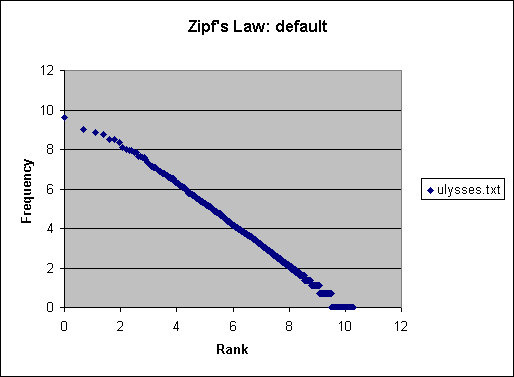
\includegraphics[width=0.5\textwidth]{ulysses_txt_default.png}
    \caption{Zipf's Law for the ``Ulysses'' corpus with the default setup.}
    \end{center}
\end{figure}

\begin{figure}
    \begin{center}
    \includegraphics[width=0.5\textwidth]{ZipfLaw_java_default.png}
    \caption{Zipf's Law for the ``ZipfLaw.java'' program itself with the default setup.}
    \end{center}
\end{figure}


\clearpage

\paragraph{Graphs, The Extreme Setup}

\begin{figure}[h!]
    \begin{center}
    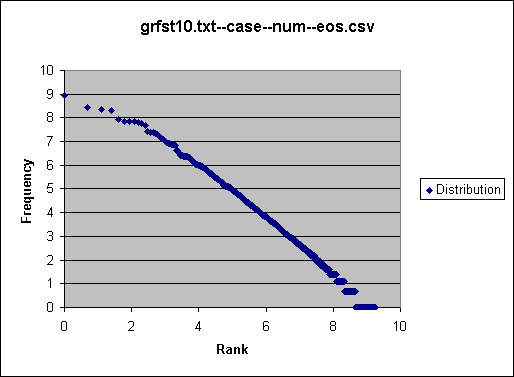
\includegraphics[width=0.5\textwidth]{grfst10_txt_case_num_eos.png}
    \caption{Zipf's Law for the ``Greifenstein'' corpus with the extreme setup.}
    \end{center}
\end{figure}

\begin{figure}
    \begin{center}
    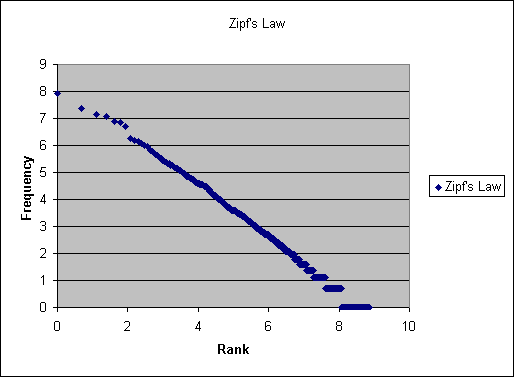
\includegraphics[width=0.5\textwidth]{hwswc10_txt_case_num_eos.png}
    \caption{Zipf's Law for the ``How to Speak and Write Correctly'' corpus with the extreme setup.}
    \end{center}
\end{figure}

\begin{figure}
    \begin{center}
    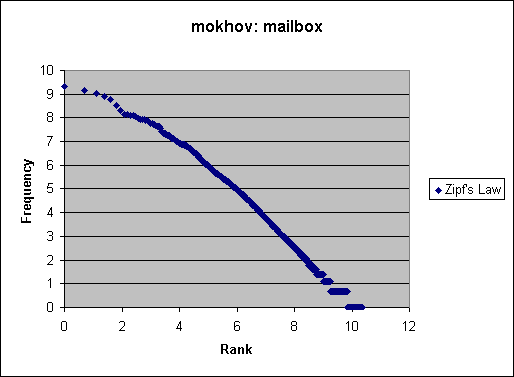
\includegraphics[width=0.5\textwidth]{mokhov_case_num_eos.png}
    \caption{Zipf's Law for my 5.6 Mb INBOX  with the extreme setup.}
    \end{center}
\end{figure}

\begin{figure}
	\begin{center}
	\includegraphics[width=0.5\textwidth]{multiprocessor_txt_case_num_eos.png}
	\caption{Zipf's Law for the white paper ``The United States Needs a Scalable Shared-Memory Multiprocessor, But Might Not Get One! with the extreme setup}
	\end{center}
\end{figure}

\begin{figure}
	\begin{center}
	\includegraphics[width=0.5\textwidth]{ulysses_txt_case_num_eos.png}
	\caption{Zipf's Law for the ``Ulysses'' corpus with the extreme setup.}
	\end{center}
\end{figure}

\begin{figure}
	\begin{center}
	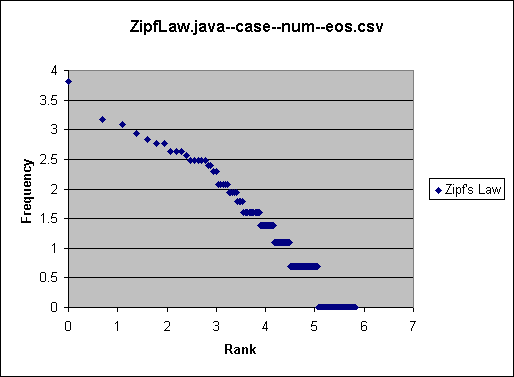
\includegraphics[width=0.5\textwidth]{ZipfLaw_java_case_num_eos.png}
	\caption{Zipf's Law for the ``ZipfLaw.java'' program itself with the extreme setup.}
	\end{center}
\end{figure}

\subsubsection{Conclusions}

Zipf's Law holds so far. However, more experimentation is required,
for example, other punctuation characters than
that ending a sentence were not considered. Then other languages than English is a good
area to explore as well.

% EOF



%
% LangIdentApp
%

\subsection{Language Identification Application}
\index{Language Identification}
\index{Language Identification!Application}
\index{Applications!Language Identification}

$Revision: 1.27 $

Originally written on March 17, 2003.

\subsubsection{The Program}

The Mini-User Manual is provided in the \xs{sect:lang-ident-app-manual}. The source
is provided in the electronic form only from the release tarballs or the CVS repository.

NOTE: in the code there are a lot of files. Not all of them might
be of a great interest to you since
some of them are stubs right now and don't provide much functionality in them
or the functionality is not linked anyhow to the main application.
These files are:

\begin{verbatim}
./marf/nlp/Collocations:
    ChiSquareTest.java
    CollocationWindow.java
    TTest.java

./marf/Stats/StatisticalEstimators:
    GLI.java
    KatzBackoff.java
    SLI.java

./marf/util/comparators:
    RankComparator.java

./marf/nlp/Stemming:
    StemmingEN.java
    Stemming.java
\end{verbatim}


\subsubsection{Hypotheses}
\index{Language Identification!Hypotheses}

\paragraph{Identifying Non-Latin-Script-Based Languages}

The methodology, if implemented correctly, should work
for natural languages that use non-Latin scripts for
their writing. Of course, to test this, such scripts
will have to be romanized (either transcribed or transliterated
using Latin, more precisely, ASCII characters).

\paragraph{Identifying Programming Languages}
\index{Language Identification!Programming Languages}

I have thought of if the proposed methodology works well for natural
languages, it would probably work at least as good for the programming
languages.

\paragraph{Sophisticated Statistical Estimators Should Work Better}

``Good'' (or ``better'' if you will) statistical estimators presented in \xc{chapt:statitstic-processing}
should give better results (higher language recognition rate) over simpler ones.
By ``simpler'' we mean the MLE and Add-* family. By more sophisticated we mean Witten-Bell,
Good-Turing, and the combination of the Statistical Estimators.

\paragraph{Zipf's Law Can Also Be Effective in Language Identification}
\index{Language Identification!Zipf's Law}
\index{Zipf's Law!Language Identification}

Zipf's Law can be reasonably effective and very ``cheap'' in language identification
task. This one is yet to be verified.

\subsubsection{Initial Experiments Setup}

\paragraph{Languages}

Several natural and programming languages in were used in the experiments.

\paragraph*{Natural Lanugages (NLs)}

\begin{itemize}
\item English (en - ISO 2-letter code code \cite{iso-codes})
\item French (fr, desaccented)
\item Spanish (es, desaccented)
\item Italian (it)
\item Arabic (ar, transcribed in ASCII according to the qalam rules \cite{qalam})
\item Hebrew (he, transcribed in ASCII)
\item Bulgarian (bg, transcribed in ASCII)
\item Russian (ru, transcribed in ASCII)
\end{itemize}

\paragraph*{Programming Languages (PLs)}

\begin{itemize}
\item {\C}/{\cpp} (together, since {\C} is a proper subset of {\cpp})
\item {\java}
\item {\perl}
\end{itemize}

\paragraph*{Statistical Estimators Implemented}

\begin{itemize}
\item MLE in \api{MLE}
\item Add-One in \api{AddOne}
\item Add-Delta (ELE) in \api{AddDelta}
\item Witten-Bell in \api{WittenBell}
\item Good-Turing in \api{GoodTuring}
\end{itemize}

\paragraph*{N-gram Models}

\begin{itemize}
\item Unigram
\item Bigram
\item Trigram
\end{itemize}

\paragraph{Corpora}

\paragraph*{English}

The English language corpora is (not very surprisingly) was the biggest one.
To simplify the training process, we combined them all in one file
\file{en.txt}. It includes
\cite{probst95, ulysses, greif, speak, fannyhill, lysistrata, canterby, defoe, rousseau, tasso}.
Additionally, a few chapters of ``The Little Prince''.
Total size of the combined file is 7Mb.

\paragraph*{French}

For French we used few chapters of ``Le Petit Prince''.
The totals combined size is 12k, \file{fr.txt}.

\paragraph*{Spanish}

Like the French corpora, the Spanish one includes several
chapters of ``Le Petit Prince'' in Spanish (from the same source).
The total size is 12k, \file{es.txt}.

\paragraph*{Arabic}

We have compiled a few surah from transliterated Quran (\cite{quran})
as well as a couple of texts transcribed by Michelle Khalif\'e
from a proverb \cite{jeha} and a passage from a newspaper in Arabic \cite{arnews}.
Total size: 208k, \file{ar.txt}.

\paragraph*{Hebrew}

We used a few poems written by their author (\cite{hepoems}) in ASCII alphabet.
Total size is 37k, \file{he.txt}.

\paragraph*{Russian}

Latinized classics (one whole book) was used (see \cite{ohotnik}).
Total size is 877k, \file{ru.txt}.

\paragraph*{Bulgarian}

A few transcribed poems were used for training from \cite{bgpoems}.
Total size: 21k, \file{bg.txt}.

\paragraph*{Italian}

We used the ``Pinocchio'' book \cite{pinocchio} of the size of 245k, \file{it.txt}.

\paragraph*{C/C++}

Various \file{.c} and \file{.cpp} files were used from a variety of projects
and examples for the ``COMP444 - System Software Design'', ``COMP471 - Computer Graphics'',
``COMP361'', and ``COMP229 - System Software courses''. The total size is 137k, \file{cpp.txt}.

\paragraph*{Java}

As Java ``corpora'' we used the sources of this application at some point in the
development cycle and source files for the MARF project itself.
The total size is 260k, \file{java.txt}.

\paragraph*{Perl}

For {\perl}, we used many of Serguei's scripts written to help with marking of
assignments and accept electronic submissions as well as a couple tools
for CVS written in {\perl} from the Internet (Google keywords: \tool{cvs2cl.pl} and \tool{cvs2html.pl}).
Size: 299k, \file{perl.txt}.

%%%%%%%%%%%%%%%%%%%%%%%%%%%%%%%%%%%%%%%%%%%%%%%
%%%%%%%%%%%%%%%%%%%%%%%%%%%%%%%%%%%%%%%%%%%%%%%

\subsubsection{Methodology}

\paragraph{Add-Delta Family}

Add-Delta is defined as:

$P(\mbox{ngram}) = \frac{C_{\mbox{ngram}} + \delta}{N + \delta \cdot V}$

\noindent
where $V$ is a vocabulary size, $N$ is the number of n-grams that start with {\em ngram}.
By implementing this general Add-Delta smoothing we get MLE, ELE, and Add-One ``for free''
as special cases of Add-Delta:

\begin{itemize}
\item $\delta = 0$ is MLE
\item $\delta = 1$ is Add One
\item $\delta = 0.5$ is ELE
\end{itemize}

\paragraph{Witten-Bell and Good Turing}

These two estimators were implemented as given in hopes to get a better
recognition rate over the Add-Delta family.

\subsubsection{Difficulties Encountered}

During the experimentations we faced several problems, some of which
are worth mentioning.

\paragraph{``Bag-of-Languages'' and Alphabets}

From this point now on, by an {\em alphabet} in this document we mean something more than what people understand
by the language alphabet. In our case an alphabet may include
characters other than letters, such as numbers, punctuation, even
a blank sometimes, all being derived from a training corpus.

Initially, we attempted to treat programming languages as if they
were natural ones. That way, from the developer's standpoint we deal with
them all uniformly. This assumption could be viewed as cheating
to some extent however because programming languages have a lot larger
alphabets that are necessary lexical parts of the language in addition
to the statements written using ASCII letters. Therefore, this gives a lot of
discriminatory power as compared to the NLs when these characters are
inputted by an user. Treating PLs as using
only ASCII Latin base should lead to a lot
of confusion with English (and sometimes other NLs) because most of the keywords
are English words in addition to literal text strings and comments present within the code.

Among NLs that were transcribed or transliterated in Latin there are alphabetical differences.
For instance, in Arabic there are three h-like sounds that have no
English equivalent, so sometimes numbers 3, 7, and 5 are used for that purpose (or in more
standard LAiLA notation \cite{qalam} capitals are used instead. To be
more fair to others, we let numerals to be a part of the alphabet as well.
Analogous problem existed when using capitals for different sounds as opposed
to direct lowercase transliteration in Arabic making lowercasing
a not necessarily good idea.

Russian and Bulgarian (transcribed from Cyrillic scripts) use
(') and some other symbols (like ([) or (]) in Bulgarian) to represent
certain letters or sounds; hence, they always have to be a part of the
alphabet.
This has caused some problems again, and I thought of another separation that is
needed: Latin-based, Cyrillic-based, and Semitic-based languages,
and our ``bag-of-languages'' approach might no do so well. (We, however, just split
PLs, Latin-based and non-Latin as the end result.)

Even for Latin-based languages that can be a problem. For example, the
letter $k$ does not exist in Spanish or Italian (it may if referred to
the foreign words, such as ``kilogram'' or proper names but is not used otherwise).
So are $w$ and $x$ and maybe some others. The same
with French~--~the letters $k$ and $w$ are very rare (so they didn't happen to be in ``Le Petit
Prince'' corpus used, for example).

\paragraph{Alphabet Normalization}

We {\em do} get different alphabet sizes
of my corpora for a language. The alphabets are derived from the corpora
themselves, so depending on the size some characters that appear in
one corpora might not appear in another. Thus, when we perform classification
task for a given sentence, the models compared may be with differently-sized
alphabets thereby returning a probability of 0.0 for the n-gram's characters that
have not been present yet in a given trained model. This can
be viewed as a non-uniform smoothing of the models and implies necessity
of the normalization of the alphabets of all the language models after
accounting for n-grams has been made, and only then smooth.

Language model normalization in has not been implemented yet. Such normalization, however, will
provoke a problem of data sparseness similar to the one described below.
This presents a problem for smoothing techniques, because some counts
we get, $N$ of either n-grams or (n-1)-grams, will have values of 0.0 and
division by 0.0 will become a problem.

\paragraph{N-grams with $n > 2$}

The implemented maximum so far is $n = 3$, but it is a general problem for any $n$.
The problem stems from
the excessive data sparseness of the models for $n > 2$. Taking for
example MLE~---~it won't be able to cope with it properly without
special care because $N$ there is now a two-dimensional matrix,
which can easily be 0.0 in places and the division by zero is unavoidable.
Analogous problem exists in the Good-Turing smoothing.
To solve this we have said if $N = 0$ make $N=1$. Maybe by doing
so (as this is a quite a kludge) we have created more trouble,
but that was the ``design decision'' in the first implementation.

\subsubsection{Experiments}

\paragraph{Bag-of-Languages and the Language Split}

We came up with a few testing sentences/statements for all languages
(can be found in the \file{test.langs} file, see \xf{fig:lang-ident-sentences}).
Then, based on my random observations above we conducted more guided experiments.

\begin{figure}\small
\hrule\vskip4pt
\input{test.langs.tex}
\caption{Sample sentences in various languages used for testing. Was used in ``Bag-of-Languages'' experiments.}
\label{fig:lang-ident-sentences}
\vskip4pt\hrule
\end{figure}

\begin{figure}\small
\hrule\vskip4pt
\input{test.latin.langs.tex}
\caption{Subset of the sample sentences in languages with Latin base.}
\label{fig:lang-ident-latin}
\vskip4pt\hrule
\end{figure}

The sentences from the \xf{fig:lang-ident-sentences} were used as-is to pipe to
the program for classification for the bag-of-languages approach. This
file has been split into parts (see \xf{fig:lang-ident-latin}, \xf{fig:lang-ident-nonlatin},
and \xf{fig:lang-ident-pls}) to try out other approaches as well (see \xs{sect:lang-ident-training}).

\begin{figure}\small
\hrule\vskip4pt
\input{test.non-latin.langs.tex}
\caption{Subset of the sample sentences in languages with non-Latin base.}
\label{fig:lang-ident-nonlatin}
\vskip4pt\hrule
\end{figure}

\begin{figure}\small
\hrule\vskip4pt
\input{test.pls.langs.tex}
\caption{Subset of the sample statements in programming languages.}
\label{fig:lang-ident-pls}
\vskip4pt\hrule
\end{figure}

\paragraph{Tokenization}

We used two types of tokenizer, {\bf restricted} and {\bf unrestricted} to experiment with
the diverse alphabets.
The ``restricted tokenizer'' means lowercase-folded ASCII characters and numbers (more corresponding
to the original requirements). The ``unrestricted tokenizer''
means additional characters are allowed and it is case-sensitive.
In both tokenizers blanks are discarded.
An implementation of these tokenizer settings via command-line options is still a TODO,
so we were simply changing the code and recompiling. The code has an unrestricted tokenizer
(\file{NLPStreamTokenizer.java} under \file{marf/nlp/util}).


\subsubsection{Training}
\label{sect:lang-ident-training}

We trained language models to include the following:

\begin{itemize}
\item all the languages (both NLs and PLs) with the restricted tokenizer
\item all the languages with the unrestricted tokenizer
\item latin-based NLs (English, French, Spanish, and Italian) with the restricted tokenizer
\item non-latin-based romanized NLs (Arabic, Hebrew, Russian, and Bulgarian) with the unrestricted tokenizer
\item PLs ({\java}, {\C}/{\cpp}, {\perl}) with the unrestricted tokenizer.
\end{itemize}


%%%%%%%%%%%%%%%%%%%%%%%%%%%%%%%%%%%%%%%%%%%%%%%%%%%%%
%%%%%%%%%%%%%%%%%%%%%%%%%%%%%%%%%%%%%%%%%%%%%%%%%%%%%

\subsubsection{Results}

\paragraph{Brief Summary}

(Brief because there's more elaborate Conclusion section).

So far, the results are good in places, sometimes pitiful.
Trigrams alone generally were very poor and slow for us.
Unigrams and bigrams performed quite well, however.

More detailed results can be observed in the \xa{sect:lang-classification-results}.
Below are the numbers as a recognition rate of the
sentences presented earlier for every language model.
Note that numbers by themselves may not convey
enough information, one has to look at the detailed results further
to actually realize that the number of samples is debatable
to be good and so are the training corpora is not
uniform. One might also want to look which languages
get confused with each other.

\paragraph{Summary of Recognition Rates}

\vspace{15pt}
\hrule
\vspace{15pt}

Language Model:

\begin{itemize}
\item ``Bag-of-Languages''
\item Unrestricted tokenizer
\end{itemize}

\begin{verbatim}
                 unigram  bigram  trigram

MLE              54.17%   16.67%  16.67%
add-delta (ELE ) 58.33%   12.50%  16.67%
add-one          58.33%   12.50%  16.67%
Witten-Bell      16.67%   29.17%  16.67%
Good-Turing      16.67%   12.50%  16.67%
\end{verbatim}

\vspace{15pt}
\hrule
\vspace{15pt}

Language Model:

\begin{itemize}
\item NLs transcribed in ASCII (Arabic, Hebrew, Bulgarian, and Russian)
\item Unrestricted tokenizer
\end{itemize}

\begin{verbatim}
                 unigram  bigram  trigram

MLE              66.67%   33.33%  33.33%
add-delta (ELE)  77.78%   11.11%  55.56%
add-one          77.78%   11.11%  55.56%
Witten-Bell      55.56%   66.67%  33.33%
Good-Turing      55.56%   55.56%  55.56%
\end{verbatim}

\vspace{15pt}
\hrule
\vspace{15pt}

Language Model:

\begin{itemize}
\item PLs only ({\C}/{\cpp}, {\java}, and {\perl})
\item Unrestricted tokenizer
\end{itemize}

\begin{verbatim}
                 unigram  bigram  trigram

MLE              33.33%   33.33%  33.33%
add-delta (ELE)  33.33%   50.00%  33.33%
add-one          33.33%   50.00%  33.33%
Witten-Bell      33.33%   50.00%  33.33%
Good-Turing      33.33%   33.33%  33.33%
\end{verbatim}

\vspace{15pt}
\hrule
\vspace{15pt}

Language Model:

\begin{itemize}
\item Latin-based Langauges only (English, French, Spanish, and Italian)
\item Restricted tokenizer
\end{itemize}

\begin{verbatim}
                 unigram  bigram  trigram

MLE              77.78%   33.33%  44.44%
add-delta (ELE)  77.78%   44.44%  55.56%
add-one          77.78%   55.56%  55.56%
Witten-Bell      44.44%   44.44%  44.44%
Good-Turing      44.44%   44.44%  55.56%
\end{verbatim}

\vspace{15pt}
\hrule
\vspace{15pt}

Language Model:

\begin{itemize}
\item ``Bag-of-Languages''
\item Restricted tokenizer
\end{itemize}

\begin{verbatim}
                 unigram  bigram  trigram

MLE              62.50%   16.67%  16.67%
add-delta (ELE)  62.50%    4.17%  12.50%
add-one          62.50%    8.33%  12.50%
Witten-Bell      16.67%   33.33%  16.67%
Good-Turing      16.67%   20.83%  25.00%
\end{verbatim}


%\subsubsection{Sample Interactive Run}

%\scriptsize
%\input{lang-ident-app-sample-run}
%\normalsize


\subsubsection{Conclusions}

\paragraph{Concrete Points}

\begin{itemize}

\item
The best results we've got so far from simpler language models;
especially using languages with the Latin base only.

\item
The methodology did work for non-Latin languages as well. Not 100\% of the time,
but around 60\%, but this is a start.

\item
Witten-Bell and Good-Turing performed rather poorly in our tests in general.
We think we need a lot larger corpora to test out Witten-Bell and Good-Turing
smoothing more thoroughly. This can be confirmed by some of the results
where Good-Turing gave us all English and English is the biggest
corpus we've got.

\item
Identification of the Latin-based languages among themselves was the best one.
It worked OK in the bag-of-languages approach.

\item
The strict tokenizer and bag-of-languages were surprisingly good (or at least
better than we expected).

\item
Recognition of the programming languages according to the conducted
experiments can be qualified as ``so-so'' when PLs are compared to
each other only. They were recognized slightly better in the bag-of-languages
approach (due to the larger alphabets).

\end{itemize}

\paragraph{Generalities}

Some of the hypotheses didn't hold (``better techniques would do better'' and
``PLs can be identified as easily as NLs''),
some didn't have time allotted to them yet (``try out Zipf's Law for the purpose
of the language identification'').

In the next releases, we want to experiment with more things, for example,
cross-validation and held-out estimation as well as
linear interpolations and Katz Backoff.


\subsubsection{Mini User Manual}
\label{sect:lang-ident-app-manual}

\paragraph{System Requirements}

The application was primarily developed under Linux, so there's
a \file{Makefile} and a testing shell script to simplify some routine tasks.
For JVM, any JDK 1.4.* and above will do. \tool{tcsh} would be nice
to have to be able to run the batch script. Since the application
itself is written in {\java}, it's not bound to specific architecture,
thus may be compiled and run without the makefiles and scripts
on virtually any operating system.

\paragraph{How To Run It}

In order for the below to work you'd need some corpora in
the same directory as the application. (Check the reference
section for the corpora used in the experiments.)
There are thousands of ways how to run the program. Some of them are listed below.

\paragraph{Using the Shell Scripts}

There are two scripts out there -- \tool{training.sh} and \tool{testing.sh}.
The former is used to do batch training on all the languages and all the models,
the latter to perform batch-testing of the models. They hide the complexity
of typing many options to the users. If you are ever to use them, tweak
them appropriately for the specific languages and n-gram models if you don't
all all-or-nothing testing.

The scripts are written using the \tool{tcsh} syntax; hence, \tool{tcsh} should be
present. The scripts ensure
that the program was compiled first, by invoking \tool{make}, then
in several \verb+for()+ loops feed all the options and filenames to the application.

Type:

\noindent
\verb+./training.sh+

to train the models.

\noindent
\verb+./testing.sh+

to test the models. NOTE: to start testing right away, you need the \file{*.gzbin} files
(pre-trained models) which should be copied from a \file{training-*} directory
of your choice to the application's directory.

\paragraph{Running The LangIdentApp Application}
\label{sect:lang-ident-app}

You can run the application itself without any wrapping scripts
and provide options to it. This is a command-line application,
so there is no GUI associated with it yet (next release). To run the application
you have to compile it first. You can use either \tool{make} with no
arguments to compile or use a standard Java compiler.

\noindent
\tool{make}

or

\noindent
\verb+javac -cp marf.jar:. LangIdentApp.java+

After having compiled the application, you can run it with the JVM.
There are several required options:

\begin{itemize}
\item
\verb+-char+ makes sure we deal with characters instead of strings of characters as a part of an n-gram

\item
one of the statistical estimators (see below); if none present, it won't pick any default one

\item
language parameter (it may seem awkward to require it for identification, but this will fixed,
so for now use anything for it, like ``foo''). Thus, the ``language'' is a typically two-to-four letter
abbrieviation of the language you are trying to train on (w.g. ``en'', ``es'', ``java'', etc.).

\item
corpus - a path to the corpus file for training. For testing just use ``bar''.
\end{itemize}

If you want an interactive mode to enter sentences yourself, use the \verb+-interactive+
option. E.g.:

\verb+java -cp marf.jar:. LangIdentApp --ident -char -interactive -bigram -add-delta foo bar+

Here are the options as per the application's output:

\vspace{15pt}
\hrule
\begin{verbatim}

Language Identification Application, $Revision: 1.1 $, $Date: 2006/02/13 14:46:56 $
Serguei A. Mokhov, mokhov@cs.concordia.ca
March 2003 - 2006


Usage:
    java LangIdentApp --help | -h
    java LangIdentApp --version
    java LangIdentApp --train [ --debug ] [ OPTIONS ] <language> <corpus-file>
    java LangIdentApp --ident [ --debug ] [ OPTIONS ] foo <bar|corpus-file>

Options (one or more of the following):
    -interactive   interactive mode for classification instead of reading from a file
    -char          use characters as n-grams (should always be present for this app)

    -unigram       use UNIGRAM model
    -bigram        use BIGRAM model
    -trigram       use TRIGRAM model

    -mle           use MLE
    -add-one       use Add-One smoothing
    -add-delta     use Add-Delta (ELE, d=0.5) smoothing
    -witten-bell   use Witten-Bell smoothing
    -good-turing   use Good-Turing smoothing

\end{verbatim}

\hrule
\vspace{15pt}

If the filename isn't specified, that will be stated and the usage
instructions above displayed.

\subsubsection{List of Files}

\paragraph{Directories}

\begin{itemize}

\item
\file{marf/nlp} -- that's where most of the code is for for use by this application, the \api{marf.nlp} package.
As discussed at the beginning, it has all the possible implementation files, but some of them are just
unimplemented stubs.

\item
\file{index/} -- this directory contains indexing of file names of corpora per language
(see \xs{sect:corpora-per-language})

\item
\file{test/} -- this directory contains testing files with sentences in various languages for testing
(see \xs{sect:lang-test-sentences})

\item
\file{expected/} -- this directory contains expected output files for classification
(see \xs{sect:lang-expected-classification})

%\item
%\file{corpora/} -- this directory contains all the corpora I had collected

\item
\file{training-*/} -- these directories contain all pre-trained models by us
for the described experiments and will be supplied in the training-sets tarballs.

\end{itemize}


\paragraph{Corpora per Language}
\label{sect:corpora-per-language}

The below is the list of files of ``pointers''
to the training corpora %under the \verb+/corpora+ directory
for the corresponding languages.

\begin{verbatim}
ar.train.corpora
bg.train.corpora
cpp.train.corpora
en.train.corpora
es.train.corpora
fr.train.corpora
he.train.corpora
it.train.corpora
java.train.corpora
perl.train.corpora
ru.train.corpora
\end{verbatim}


\paragraph{Expected Results}
\label{sect:lang-expected-classification}

The below files present the ideal results of batch
identification that correspond the \file{test.*.langs} files below,
and can be compared to those produced by the \tool{testing.sh} script.

\begin{verbatim}
expected.langs
expected.latin.langs
expected.non-latin.langs
expected.pls.langs
\end{verbatim}


\paragraph{Application}

The application and its makefile.

\begin{verbatim}
LangIdentApp.java
Makefile
marf.jar
\end{verbatim}


\paragraph{Scripts}

The wrapper scripts for batch training and testing.

\begin{verbatim}
testing.sh
training.sh
\end{verbatim}


\paragraph{Test Sentences}
\label{sect:lang-test-sentences}

\begin{itemize}
\item
\file{test.langs} --- the bag-of-languages

\item
\file{test.latin.langs} --- English, French, Spanish, and Italian sentences

\item
\file{test.non-latin.langs} --- Arabic, Hebrew, Russian, and Bulgarian sentences

\item
\file{test.pls.langs} --- Programming Languages (a few statements in {\cpp}, {\java}, and {\perl})
\end{itemize}


%%%%%%%%%%%%%%%%%%%%%%%%%%%%%%%%%%%%%%%%%%%%%%%%%%%%
%%%%%%%%%%%%%%%%%%%%%%%%%%%%%%%%%%%%%%%%%%%%%%%%%%%%

\subsubsection{Classification Results}
\label{sect:lang-classification-results}

\paragraph{``Bag-of-Languages'', Unrestricted Tokenizer}

\tiny
\hrule\vskip4pt
\begin{verbatim}
UNIGRAM, ADD-DELTA                                                 UNIGRAM, ADD-ONE

Ideal                        Actual                       Match    Ideal                        Actual                       Match

Language identified: [en]    Language identified: [en]    1        Language identified: [en]    Language identified: [en]    1
Language identified: [en]    Language identified: [en]    2        Language identified: [en]    Language identified: [en]    2
Language identified: [es]    Language identified: [fr]             Language identified: [es]    Language identified: [fr]
Language identified: [en]    Language identified: [en]    3        Language identified: [en]    Language identified: [en]    3
Language identified: [ru]    Language identified: [ru]    4        Language identified: [ru]    Language identified: [ru]    4
Language identified: [fr]    Language identified: [fr]    5        Language identified: [fr]    Language identified: [fr]    5
Language identified: [ru]    Language identified: [ru]    6        Language identified: [ru]    Language identified: [ru]    6
Language identified: [es]    Language identified: [es]    7        Language identified: [es]    Language identified: [es]    7
Language identified: [he]    Language identified: [he]    8        Language identified: [he]    Language identified: [he]    8
Language identified: [it]    Language identified: [it]    9        Language identified: [it]    Language identified: [it]    9
Language identified: [ar]    Language identified: [ru]             Language identified: [ar]    Language identified: [ru]
Language identified: [bg]    Language identified: [bg]    10       Language identified: [bg]    Language identified: [bg]    10
Language identified: [java]  Language identified: [es]             Language identified: [java]  Language identified: [es]
Language identified: [cpp]   Language identified: [perl]           Language identified: [cpp]   Language identified: [perl]
Language identified: [cpp]   Language identified: [perl]           Language identified: [cpp]   Language identified: [perl]
Language identified: [he]    Language identified: [he]    11       Language identified: [he]    Language identified: [he]    11
Language identified: [java]  Language identified: [it]             Language identified: [java]  Language identified: [it]
Language identified: [perl]  Language identified: [cpp]            Language identified: [perl]  Language identified: [cpp]
Language identified: [ar]    Language identified: [ar]    12       Language identified: [ar]    Language identified: [ar]    12
Language identified: [perl]  Language identified: [es]             Language identified: [perl]  Language identified: [es]
Language identified: [ru]    Language identified: [ru]    13       Language identified: [ru]    Language identified: [ru]    13
Language identified: [fr]    Language identified: [it]             Language identified: [fr]    Language identified: [it]
Language identified: [ar]    Language identified: [bg]             Language identified: [ar]    Language identified: [bg]
Language identified: [en]    Language identified: [en]    14       Language identified: [en]    Language identified: [en]    14

Total                        24                           14       Total                        24                           14
%                            58.33                                 %                            58.33
\end{verbatim}
\vskip4pt\hrule

\clearpage

\tiny
\hrule\vskip4pt
\begin{verbatim}
UNIGRAM, GOOD-TURING                                               UNIGRAM, MLE

Ideal                        Actual                       Match    Ideal                        Actual                       Match

Language identified: [en]    Language identified: [en]    1        Language identified: [en]    Language identified: [en]    1
Language identified: [en]    Language identified: [en]    2        Language identified: [en]    Language identified: [en]    2
Language identified: [es]    Language identified: [en]             Language identified: [es]    Language identified: [fr]
Language identified: [en]    Language identified: [en]    3        Language identified: [en]    Language identified: [en]    3
Language identified: [ru]    Language identified: [en]             Language identified: [ru]    Language identified: [bg]
Language identified: [fr]    Language identified: [en]             Language identified: [fr]    Language identified: [fr]    4
Language identified: [ru]    Language identified: [en]             Language identified: [ru]    Language identified: [ru]    5
Language identified: [es]    Language identified: [en]             Language identified: [es]    Language identified: [es]    6
Language identified: [he]    Language identified: [en]             Language identified: [he]    Language identified: [he]    7
Language identified: [it]    Language identified: [en]             Language identified: [it]    Language identified: [it]    8
Language identified: [ar]    Language identified: [en]             Language identified: [ar]    Language identified: [ru]
Language identified: [bg]    Language identified: [en]             Language identified: [bg]    Language identified: [bg]    9
Language identified: [java]  Language identified: [en]             Language identified: [java]  Language identified: [es]
Language identified: [cpp]   Language identified: [en]             Language identified: [cpp]   Language identified: [perl]
Language identified: [cpp]   Language identified: [en]             Language identified: [cpp]   Language identified: [perl]
Language identified: [he]    Language identified: [en]             Language identified: [he]    Language identified: [he]    10
Language identified: [java]  Language identified: [en]             Language identified: [java]  Language identified: [it]
Language identified: [perl]  Language identified: [en]             Language identified: [perl]  Language identified: [cpp]
Language identified: [ar]    Language identified: [en]             Language identified: [ar]    Language identified: [ar]    11
Language identified: [perl]  Language identified: [en]             Language identified: [perl]  Language identified: [es]
Language identified: [ru]    Language identified: [en]             Language identified: [ru]    Language identified: [ru]    12
Language identified: [fr]    Language identified: [en]             Language identified: [fr]    Language identified: [it]
Language identified: [ar]    Language identified: [en]             Language identified: [ar]    Language identified: [bg]
Language identified: [en]    Language identified: [en]    4        Language identified: [en]    Language identified: [en]    13

Total                        24                           4        Total                        24                           13
%                            16.67                                 %                            54.17
\end{verbatim}
\vskip4pt\hrule


\tiny
\hrule\vskip4pt
\begin{verbatim}
UNIGRAM, WITTEN-BELL                                               BIGRAM, ADD-DELTA

Ideal                        Actual                       Match    Ideal                        Actual                       Match

Language identified: [en]    Language identified: [en]    1        Language identified: [en]    Language identified: [bg]
Language identified: [en]    Language identified: [en]    2        Language identified: [en]    Language identified: [fr]
Language identified: [es]    Language identified: [en]             Language identified: [es]    Language identified: [es]    1
Language identified: [en]    Language identified: [en]    3        Language identified: [en]    Language identified: [bg]
Language identified: [ru]    Language identified: [en]             Language identified: [ru]    Language identified: [bg]
Language identified: [fr]    Language identified: [en]             Language identified: [fr]    Language identified: [fr]    2
Language identified: [ru]    Language identified: [en]             Language identified: [ru]    Language identified: [bg]
Language identified: [es]    Language identified: [en]             Language identified: [es]    Language identified: [fr]
Language identified: [he]    Language identified: [en]             Language identified: [he]    Language identified: [bg]
Language identified: [it]    Language identified: [en]             Language identified: [it]    Language identified: [fr]
Language identified: [ar]    Language identified: [en]             Language identified: [ar]    Language identified: [fr]
Language identified: [bg]    Language identified: [en]             Language identified: [bg]    Language identified: [es]
Language identified: [java]  Language identified: [en]             Language identified: [java]  Language identified: [fr]
Language identified: [cpp]   Language identified: [en]             Language identified: [cpp]   Language identified: [perl]
Language identified: [cpp]   Language identified: [en]             Language identified: [cpp]   Language identified: [cpp]   3
Language identified: [he]    Language identified: [en]             Language identified: [he]    Language identified: [bg]
Language identified: [java]  Language identified: [en]             Language identified: [java]  Language identified: [fr]
Language identified: [perl]  Language identified: [en]             Language identified: [perl]  Language identified: [es]
Language identified: [ar]    Language identified: [en]             Language identified: [ar]    Language identified: [bg]
Language identified: [perl]  Language identified: [en]             Language identified: [perl]  Language identified: [fr]
Language identified: [ru]    Language identified: [en]             Language identified: [ru]    Language identified: [bg]
Language identified: [fr]    Language identified: [en]             Language identified: [fr]    Language identified: [es]
Language identified: [ar]    Language identified: [en]             Language identified: [ar]    Language identified: [es]
Language identified: [en]    Language identified: [en]    4        Language identified: [en]    Language identified: [bg]

Total                        24                           4        Total                        24                           3
%                            16.67                                 %                            12.50
\end{verbatim}
\vskip4pt\hrule

\clearpage

\tiny
\hrule\vskip4pt
\begin{verbatim}
BIGRAM,ADD-ONE                                                     BIGRAM, GOOD-TURING

Ideal                        Actual                       Match    Ideal                        Actual                       Match

Language identified: [en]    Language identified: [bg]             Language identified: [en]    Language identified: [en]    1
Language identified: [en]    Language identified: [fr]             Language identified: [en]    Language identified: [perl]
Language identified: [es]    Language identified: [es]    1        Language identified: [es]    Language identified: [perl]
Language identified: [en]    Language identified: [bg]             Language identified: [en]    Language identified: [perl]
Language identified: [ru]    Language identified: [bg]             Language identified: [ru]    Language identified: [perl]
Language identified: [fr]    Language identified: [fr]    2        Language identified: [fr]    Language identified: [perl]
Language identified: [ru]    Language identified: [bg]             Language identified: [ru]    Language identified: [perl]
Language identified: [es]    Language identified: [fr]             Language identified: [es]    Language identified: [perl]
Language identified: [he]    Language identified: [bg]             Language identified: [he]    Language identified: [perl]
Language identified: [it]    Language identified: [fr]             Language identified: [it]    Language identified: [perl]
Language identified: [ar]    Language identified: [fr]             Language identified: [ar]    Language identified: [perl]
Language identified: [bg]    Language identified: [es]             Language identified: [bg]    Language identified: [perl]
Language identified: [java]  Language identified: [fr]             Language identified: [java]  Language identified: [perl]
Language identified: [cpp]   Language identified: [perl]           Language identified: [cpp]   Language identified: [perl]
Language identified: [cpp]   Language identified: [cpp]   3        Language identified: [cpp]   Language identified: [perl]
Language identified: [he]    Language identified: [bg]             Language identified: [he]    Language identified: [perl]
Language identified: [java]  Language identified: [fr]             Language identified: [java]  Language identified: [perl]
Language identified: [perl]  Language identified: [es]             Language identified: [perl]  Language identified: [perl]  2
Language identified: [ar]    Language identified: [bg]             Language identified: [ar]    Language identified: [perl]
Language identified: [perl]  Language identified: [fr]             Language identified: [perl]  Language identified: [perl]  3
Language identified: [ru]    Language identified: [bg]             Language identified: [ru]    Language identified: [perl]
Language identified: [fr]    Language identified: [es]             Language identified: [fr]    Language identified: [perl]
Language identified: [ar]    Language identified: [es]             Language identified: [ar]    Language identified: [perl]
Language identified: [en]    Language identified: [bg]             Language identified: [en]    Language identified: [perl]

Total                        24                           3        Total                        24                           3
%                            12.50                                 %                            12.50
\end{verbatim}
\vskip4pt\hrule


\tiny
\hrule\vskip4pt
\begin{verbatim}
BIGRAM, MLE                                                        BIGRAM, WITTEN-BELL

Ideal                        Actual                       Match    Ideal                        Actual                       Match

Language identified: [en]    Language identified: [en]    1        Language identified: [en]    Language identified: [java]
Language identified: [en]    Language identified: [en]    2        Language identified: [en]    Language identified: [java]
Language identified: [es]    Language identified: [en]             Language identified: [es]    Language identified: [es]    1
Language identified: [en]    Language identified: [en]    3        Language identified: [en]    Language identified: [java]
Language identified: [ru]    Language identified: [en]             Language identified: [ru]    Language identified: [java]
Language identified: [fr]    Language identified: [en]             Language identified: [fr]    Language identified: [es]
Language identified: [ru]    Language identified: [en]             Language identified: [ru]    Language identified: [java]
Language identified: [es]    Language identified: [en]             Language identified: [es]    Language identified: [ar]
Language identified: [he]    Language identified: [en]             Language identified: [he]    Language identified: [ar]
Language identified: [it]    Language identified: [en]             Language identified: [it]    Language identified: [it]    2
Language identified: [ar]    Language identified: [en]             Language identified: [ar]    Language identified: [ar]    3
Language identified: [bg]    Language identified: [en]             Language identified: [bg]    Language identified: [java]
Language identified: [java]  Language identified: [en]             Language identified: [java]  Language identified: [es]
Language identified: [cpp]   Language identified: [en]             Language identified: [cpp]   Language identified: [java]
Language identified: [cpp]   Language identified: [en]             Language identified: [cpp]   Language identified: [cpp]   4
Language identified: [he]    Language identified: [en]             Language identified: [he]    Language identified: [ru]
Language identified: [java]  Language identified: [en]             Language identified: [java]  Language identified: [java]  5
Language identified: [perl]  Language identified: [en]             Language identified: [perl]  Language identified: [ru]
Language identified: [ar]    Language identified: [en]             Language identified: [ar]    Language identified: [ar]    6
Language identified: [perl]  Language identified: [en]             Language identified: [perl]  Language identified: [java]
Language identified: [ru]    Language identified: [en]             Language identified: [ru]    Language identified: [ar]
Language identified: [fr]    Language identified: [en]             Language identified: [fr]    Language identified: [java]
Language identified: [ar]    Language identified: [en]             Language identified: [ar]    Language identified: [ar]    7
Language identified: [en]    Language identified: [en]    4        Language identified: [en]    Language identified: [java]

Total                        24                           4        Total                        24                           7
%                            16.67                                 %                            29.17
\end{verbatim}
\vskip4pt\hrule

\clearpage

\tiny
\hrule\vskip4pt
\begin{verbatim}
TRIGRAM, ADD-DELTA                                                 TRIGRAM, ADD-ONE

Ideal                        Actual                       Match    Ideal                        Actual                       Match

Language identified: [en]    Language identified: [he]             Language identified: [en]    Language identified: [he]
Language identified: [en]    Language identified: [fr]             Language identified: [en]    Language identified: [fr]
Language identified: [es]    Language identified: [fr]             Language identified: [es]    Language identified: [fr]
Language identified: [en]    Language identified: [he]             Language identified: [en]    Language identified: [he]
Language identified: [ru]    Language identified: [he]             Language identified: [ru]    Language identified: [he]
Language identified: [fr]    Language identified: [fr]    1        Language identified: [fr]    Language identified: [fr]    1
Language identified: [ru]    Language identified: [he]             Language identified: [ru]    Language identified: [he]
Language identified: [es]    Language identified: [fr]             Language identified: [es]    Language identified: [fr]
Language identified: [he]    Language identified: [ar]             Language identified: [he]    Language identified: [ar]
Language identified: [it]    Language identified: [fr]             Language identified: [it]    Language identified: [fr]
Language identified: [ar]    Language identified: [fr]             Language identified: [ar]    Language identified: [fr]
Language identified: [bg]    Language identified: [fr]             Language identified: [bg]    Language identified: [fr]
Language identified: [java]  Language identified: [fr]             Language identified: [java]  Language identified: [fr]
Language identified: [cpp]   Language identified: [java]           Language identified: [cpp]   Language identified: [java]
Language identified: [cpp]   Language identified: [java]           Language identified: [cpp]   Language identified: [java]
Language identified: [he]    Language identified: [he]    2        Language identified: [he]    Language identified: [he]    2
Language identified: [java]  Language identified: [fr]             Language identified: [java]  Language identified: [fr]
Language identified: [perl]  Language identified: [es]             Language identified: [perl]  Language identified: [es]
Language identified: [ar]    Language identified: [ar]    3        Language identified: [ar]    Language identified: [ar]    3
Language identified: [perl]  Language identified: [fr]             Language identified: [perl]  Language identified: [fr]
Language identified: [ru]    Language identified: [ar]             Language identified: [ru]    Language identified: [ar]
Language identified: [fr]    Language identified: [fr]    4        Language identified: [fr]    Language identified: [fr]    4
Language identified: [ar]    Language identified: [fr]             Language identified: [ar]    Language identified: [fr]
Language identified: [en]    Language identified: [he]             Language identified: [en]    Language identified: [he]

Total                        24                           4        Total                        24                           4
%                            16.67                                 %                            16.67
\end{verbatim}
\vskip4pt\hrule


\tiny
\hrule\vskip4pt
\begin{verbatim}
TRIGRAM, GOOD-TURING                                               TRIGRAM, MLE

Ideal                        Actual                       Match    Ideal                        Actual                       Match

Language identified: [en]    Language identified: [he]             Language identified: [en]    Language identified: [en]    1
Language identified: [en]    Language identified: [he]             Language identified: [en]    Language identified: [en]    2
Language identified: [es]    Language identified: [ar]             Language identified: [es]    Language identified: [en]
Language identified: [en]    Language identified: [he]             Language identified: [en]    Language identified: [en]    3
Language identified: [ru]    Language identified: [he]             Language identified: [ru]    Language identified: [en]
Language identified: [fr]    Language identified: [ar]             Language identified: [fr]    Language identified: [en]
Language identified: [ru]    Language identified: [he]             Language identified: [ru]    Language identified: [en]
Language identified: [es]    Language identified: [ar]             Language identified: [es]    Language identified: [en]
Language identified: [he]    Language identified: [ar]             Language identified: [he]    Language identified: [en]
Language identified: [it]    Language identified: [he]             Language identified: [it]    Language identified: [en]
Language identified: [ar]    Language identified: [ar]    1        Language identified: [ar]    Language identified: [en]
Language identified: [bg]    Language identified: [es]             Language identified: [bg]    Language identified: [en]
Language identified: [java]  Language identified: [ru]             Language identified: [java]  Language identified: [en]
Language identified: [cpp]   Language identified: [ar]             Language identified: [cpp]   Language identified: [en]
Language identified: [cpp]   Language identified: [ar]             Language identified: [cpp]   Language identified: [en]
Language identified: [he]    Language identified: [he]    2        Language identified: [he]    Language identified: [en]
Language identified: [java]  Language identified: [he]             Language identified: [java]  Language identified: [en]
Language identified: [perl]  Language identified: [ar]             Language identified: [perl]  Language identified: [en]
Language identified: [ar]    Language identified: [ar]    3        Language identified: [ar]    Language identified: [en]
Language identified: [perl]  Language identified: [ar]             Language identified: [perl]  Language identified: [en]
Language identified: [ru]    Language identified: [ar]             Language identified: [ru]    Language identified: [en]
Language identified: [fr]    Language identified: [he]             Language identified: [fr]    Language identified: [en]
Language identified: [ar]    Language identified: [ar]    4        Language identified: [ar]    Language identified: [en]
Language identified: [en]    Language identified: [he]             Language identified: [en]    Language identified: [en]    4

Total                        24                           4        Total                        24                           4
%                            16.67                                 %                            16.67
\end{verbatim}
\vskip4pt\hrule

\clearpage

\tiny
\hrule\vskip4pt
\begin{verbatim}
TRIGRAM, WITTEN-BELL

Ideal                        Actual                       Match

Language identified: [en]    Language identified: [en]    1
Language identified: [en]    Language identified: [en]    2
Language identified: [es]    Language identified: [en]
Language identified: [en]    Language identified: [en]    3
Language identified: [ru]    Language identified: [en]
Language identified: [fr]    Language identified: [en]
Language identified: [ru]    Language identified: [en]
Language identified: [es]    Language identified: [en]
Language identified: [he]    Language identified: [en]
Language identified: [it]    Language identified: [en]
Language identified: [ar]    Language identified: [en]
Language identified: [bg]    Language identified: [en]
Language identified: [java]  Language identified: [en]
Language identified: [cpp]   Language identified: [en]
Language identified: [cpp]   Language identified: [en]
Language identified: [he]    Language identified: [en]
Language identified: [java]  Language identified: [en]
Language identified: [perl]  Language identified: [en]
Language identified: [ar]    Language identified: [en]
Language identified: [perl]  Language identified: [en]
Language identified: [ru]    Language identified: [en]
Language identified: [fr]    Language identified: [en]
Language identified: [ar]    Language identified: [en]
Language identified: [ar]    Language identified: [en]    4

Total                        24                           4
%                            16.67
\end{verbatim}
\vskip4pt\hrule

\clearpage

\paragraph{Non-Latin-Based Languages, Unrestricted Tokenizer}

\tiny
\hrule\vskip4pt
\begin{verbatim}
UNIGRAM, ADD-DELTA                                                 UNIGRAM, ADD-ONE

Ideal                        Actual                       Match    Ideal                        Actual                       Match

Language identified: [ru]    Language identified: [ru]    1        Language identified: [ru]    Language identified: [ru]    1
Language identified: [ru]    Language identified: [ru]    2        Language identified: [ru]    Language identified: [ru]    2
Language identified: [he]    Language identified: [he]    3        Language identified: [he]    Language identified: [he]    3
Language identified: [ar]    Language identified: [ru]             Language identified: [ar]    Language identified: [ru]
Language identified: [bg]    Language identified: [bg]    4        Language identified: [bg]    Language identified: [bg]    4
Language identified: [he]    Language identified: [he]    5        Language identified: [he]    Language identified: [he]    5
Language identified: [ar]    Language identified: [ar]    6        Language identified: [ar]    Language identified: [ar]    6
Language identified: [ru]    Language identified: [ru]    7        Language identified: [ru]    Language identified: [ru]    7
Language identified: [ar]    Language identified: [bg]             Language identified: [ar]    Language identified: [bg]

Total                        9                            7        Total                        9                            7
%                            77.78                                 %                            77.78
\end{verbatim}
\vskip4pt\hrule


\tiny
\hrule\vskip4pt
\begin{verbatim}
UNIGRAM, GOOD-TURING                                               UNIGRAM, MLE

Ideal                        Actual                       Match    Ideal                        Actual                       Match

Language identified: [ru]    Language identified: [ru]    1        Language identified: [ru]    Language identified: [bg]
Language identified: [ru]    Language identified: [ru]    2        Language identified: [ru]    Language identified: [ru]    1
Language identified: [he]    Language identified: [ru]             Language identified: [he]    Language identified: [he]    2
Language identified: [ar]    Language identified: [ru]             Language identified: [ar]    Language identified: [ru]
Language identified: [bg]    Language identified: [bg]    3        Language identified: [bg]    Language identified: [bg]    3
Language identified: [he]    Language identified: [ru]             Language identified: [he]    Language identified: [he]    4
Language identified: [ar]    Language identified: [ar]    4        Language identified: [ar]    Language identified: [ar]    5
Language identified: [ru]    Language identified: [ru]    5        Language identified: [ru]    Language identified: [ru]    6
Language identified: [ar]    Language identified: [ru]             Language identified: [ar]    Language identified: [bg]

Total                        9                            5        Total                        9                            6
%                            55.56                                 %                            66.67
\end{verbatim}
\vskip4pt\hrule


\tiny
\hrule\vskip4pt
\begin{verbatim}
UNIGRAM, WITTEN-BELL                                               BIGRAM, ADD-DELTA

Ideal                        Actual                       Match    Ideal                        Actual                       Match

Language identified: [ru]    Language identified: [ru]    1        Language identified: [ru]    Language identified: [bg]
Language identified: [ru]    Language identified: [ru]    2        Language identified: [ru]    Language identified: [bg]
Language identified: [he]    Language identified: [ru]             Language identified: [he]    Language identified: [bg]
Language identified: [ar]    Language identified: [ru]             Language identified: [ar]    Language identified: [bg]
Language identified: [bg]    Language identified: [bg]    3        Language identified: [bg]    Language identified: [bg]    1
Language identified: [he]    Language identified: [ru]             Language identified: [he]    Language identified: [bg]
Language identified: [ar]    Language identified: [ar]    4        Language identified: [ar]    Language identified: [bg]
Language identified: [ru]    Language identified: [ru]    5        Language identified: [ru]    Language identified: [bg]
Language identified: [ar]    Language identified: [ru]             Language identified: [ar]    Language identified: [bg]

Total                        9                            5        Total                        9                            1
%                            55.56                                 %                            11.11
\end{verbatim}
\vskip4pt\hrule


\tiny
\hrule\vskip4pt
\begin{verbatim}
BIGRAM, ADD-ONE                                                    BIGRAM, GOOD-TURING

Ideal                        Actual                       Match    Ideal                        Actual                       Match

Language identified: [ru]    Language identified: [bg]             Language identified: [ru]    Language identified: [ru]    1
Language identified: [ru]    Language identified: [bg]             Language identified: [ru]    Language identified: [ru]    2
Language identified: [he]    Language identified: [bg]             Language identified: [he]    Language identified: [ar]
Language identified: [ar]    Language identified: [bg]             Language identified: [ar]    Language identified: [ar]
Language identified: [bg]    Language identified: [bg]    1        Language identified: [bg]    Language identified: [bg]    3
Language identified: [he]    Language identified: [bg]             Language identified: [he]    Language identified: [ru]
Language identified: [ar]    Language identified: [bg]             Language identified: [ar]    Language identified: [ar]    4
Language identified: [ru]    Language identified: [bg]             Language identified: [ru]    Language identified: [ru]    5
Language identified: [ar]    Language identified: [bg]             Language identified: [ar]    Language identified: [ru]

Total                        9                            1        Total                        9                            5
%                            11.11                                 %                            55.56
\end{verbatim}
\vskip4pt\hrule

\clearpage

\tiny
\hrule\vskip4pt
\begin{verbatim}
BIGRAM, MLE                                                        BIGRAM, WITTEN-BELL

Ideal                        Actual                       Match    Ideal                        Actual                       Match

Language identified: [ru]    Language identified: [ru]    1        Language identified: [ru]    Language identified: [ru]    1
Language identified: [ru]    Language identified: [ru]    2        Language identified: [ru]    Language identified: [ru]    2
Language identified: [he]    Language identified: [ru]             Language identified: [he]    Language identified: [ar]
Language identified: [ar]    Language identified: [ru]             Language identified: [ar]    Language identified: [ar]    3
Language identified: [bg]    Language identified: [ru]             Language identified: [bg]    Language identified: [bg]    4
Language identified: [he]    Language identified: [ru]             Language identified: [he]    Language identified: [ru]
Language identified: [ar]    Language identified: [ru]             Language identified: [ar]    Language identified: [ar]    5
Language identified: [ru]    Language identified: [ru]    3        Language identified: [ru]    Language identified: [ar]
Language identified: [ar]    Language identified: [ru]             Language identified: [ar]    Language identified: [ar]    6

Total                        9                            3        Total                        9                            6
%                            33.33                                 %                            66.67
\end{verbatim}
\vskip4pt\hrule


\tiny
\hrule\vskip4pt
\begin{verbatim}
TRIGRAM, ADD-DELTA                                                 TRIGRAM, ADD-ONE

Ideal                        Actual                       Match    Ideal                        Actual                       Match

Language identified: [ru]    Language identified: [he]             Language identified: [ru]    Language identified: [he]
Language identified: [ru]    Language identified: [he]             Language identified: [ru]    Language identified: [he]
Language identified: [he]    Language identified: [ar]             Language identified: [he]    Language identified: [ar]
Language identified: [ar]    Language identified: [ar]    1        Language identified: [ar]    Language identified: [ar]    1
Language identified: [bg]    Language identified: [bg]    2        Language identified: [bg]    Language identified: [bg]    2
Language identified: [he]    Language identified: [he]    3        Language identified: [he]    Language identified: [he]    3
Language identified: [ar]    Language identified: [ar]    4        Language identified: [ar]    Language identified: [ar]    4
Language identified: [ru]    Language identified: [ar]             Language identified: [ru]    Language identified: [ar]
Language identified: [ar]    Language identified: [ar]    5        Language identified: [ar]    Language identified: [ar]    5

Total                        9                            5        Total                        9                            5
%                            55.56                                 %                            55.56
\end{verbatim}
\vskip4pt\hrule


\tiny
\hrule\vskip4pt
\begin{verbatim}
TRIGRAM, GOOD-TURING                                               TRIGRAM, MLE

Ideal                        Actual                       Match    Ideal                        Actual                       Match

Language identified: [ru]    Language identified: [he]             Language identified: [ru]    Language identified: [ru]    1
Language identified: [ru]    Language identified: [he]             Language identified: [ru]    Language identified: [ru]    2
Language identified: [he]    Language identified: [ar]             Language identified: [he]    Language identified: [ru]
Language identified: [ar]    Language identified: [ar]    1        Language identified: [ar]    Language identified: [ru]
Language identified: [bg]    Language identified: [bg]    2        Language identified: [bg]    Language identified: [ru]
Language identified: [he]    Language identified: [he]    3        Language identified: [he]    Language identified: [ru]
Language identified: [ar]    Language identified: [ar]    4        Language identified: [ar]    Language identified: [ru]
Language identified: [ru]    Language identified: [ar]             Language identified: [ru]    Language identified: [ru]    3
Language identified: [ar]    Language identified: [ar]    5        Language identified: [ar]    Language identified: [ru]

Total                        9                            5        Total                        9                            3
%                            55.56                                 %                            33.33
\end{verbatim}
\vskip4pt\hrule


\tiny
\hrule\vskip4pt
\begin{verbatim}
TRIGRAM, WITTEN-BELL

Ideal                        Actual                       Match

Language identified: [ru]    Language identified: [ru]    1
Language identified: [ru]    Language identified: [ru]    2
Language identified: [he]    Language identified: [ru]
Language identified: [ar]    Language identified: [ru]
Language identified: [bg]    Language identified: [ru]
Language identified: [he]    Language identified: [ru]
Language identified: [ar]    Language identified: [ru]
Language identified: [ru]    Language identified: [ru]    3
Language identified: [ar]    Language identified: [ru]

Total                        9                            3
%                            33.33
\end{verbatim}
\vskip4pt\hrule

\clearpage

\paragraph{Programming Languages, Unrestricted Tokenizer}

\tiny
\hrule\vskip4pt
\begin{verbatim}
UNIGRAM,ADD-DELTA                UNIGRAM,ADD-ONE

Ideal                          Actual                         Match  Ideal                          Actual                         Match

Language identified: [java]    Language identified: [java]    1      Language identified: [java]    Language identified: [java]    1
Language identified: [cpp]     Language identified: [perl]           Language identified: [cpp]     Language identified: [perl]
Language identified: [cpp]     Language identified: [perl]           Language identified: [cpp]     Language identified: [perl]
Language identified: [java]    Language identified: [java]    2      Language identified: [java]    Language identified: [java]    2
Language identified: [perl]    Language identified: [cpp]            Language identified: [perl]    Language identified: [cpp]
Language identified: [perl]    Language identified: [cpp]            Language identified: [perl]    Language identified: [cpp]

Total    6    2        Total    6    2
%    33.33            %    33.33
\end{verbatim}
\vskip4pt\hrule

\tiny
\hrule\vskip4pt
\begin{verbatim}
UNIGRAM,GOOD-TURING                UNIGRAM,MLE

Ideal                          Actual                         Match  Ideal                          Actual                         Match

Language identified: [java]    Language identified: [perl]           Language identified: [java]    Language identified: [java]    1
Language identified: [cpp]     Language identified: [perl]           Language identified: [cpp]     Language identified: [perl]
Language identified: [cpp]     Language identified: [perl]           Language identified: [cpp]     Language identified: [perl]
Language identified: [java]    Language identified: [java]    1      Language identified: [java]    Language identified: [java]    2
Language identified: [perl]    Language identified: [java]           Language identified: [perl]    Language identified: [cpp]
Language identified: [perl]    Language identified: [perl]    2      Language identified: [perl]    Language identified: [cpp]

Total    6    2        Total    6    2
%    33.33            %    33.33
\end{verbatim}
\vskip4pt\hrule

\tiny
\hrule\vskip4pt
\begin{verbatim}
UNIGRAM,WITTEN-BELL                                                  BIGRAM,ADD-DELTA

Ideal                          Actual                         Match  Ideal                          Actual                         Match

Language identified: [java]    Language identified: [perl]           Language identified: [java]    Language identified: [perl]
Language identified: [cpp]     Language identified: [perl]           Language identified: [cpp]     Language identified: [perl]
Language identified: [cpp]     Language identified: [perl]           Language identified: [cpp]     Language identified: [cpp]     1
Language identified: [java]    Language identified: [java]    1      Language identified: [java]    Language identified: [perl]
Language identified: [perl]    Language identified: [java]           Language identified: [perl]    Language identified: [perl]    2
Language identified: [perl]    Language identified: [perl]    2      Language identified: [perl]    Language identified: [perl]    3

Total                          6                              2      Total                          6                              3
%                              33.33                                 %                              50.00
\end{verbatim}
\vskip4pt\hrule

\tiny
\hrule\vskip4pt
\begin{verbatim}
BIGRAM,ADD-ONE                                                       BIGRAM,GOOD-TURING

Ideal                          Actual                         Match  Ideal                          Actual                         Match

Language identified: [java]    Language identified: [perl]           Language identified: [java]    Language identified: [perl]
Language identified: [cpp]     Language identified: [perl]           Language identified: [cpp]     Language identified: [perl]
Language identified: [cpp]     Language identified: [cpp]     1      Language identified: [cpp]     Language identified: [perl]
Language identified: [java]    Language identified: [perl]           Language identified: [java]    Language identified: [perl]
Language identified: [perl]    Language identified: [perl]    2      Language identified: [perl]    Language identified: [perl]    1
Language identified: [perl]    Language identified: [perl]    3      Language identified: [perl]    Language identified: [perl]    2

Total                          6                              3      Total                          6                              2
%                              50.00                                 %                              33.33
\end{verbatim}
\vskip4pt\hrule

\clearpage

\tiny
\hrule\vskip4pt
\begin{verbatim}
BIGRAM,MLE                                                           BIGRAM,WITTEN-BELL

Ideal                          Actual                         Match  Ideal                          Actual                         Match

Language identified: [java]    Language identified: [java]    1      Language identified: [java]    Language identified: [java]    1
Language identified: [cpp]     Language identified: [java]           Language identified: [cpp]     Language identified: [java]
Language identified: [cpp]     Language identified: [java]           Language identified: [cpp]     Language identified: [cpp]     2
Language identified: [java]    Language identified: [java]    2      Language identified: [java]    Language identified: [java]    3
Language identified: [perl]    Language identified: [java]           Language identified: [perl]    Language identified: [java]
Language identified: [perl]    Language identified: [java]           Language identified: [perl]    Language identified: [java]

Total                          6                              2      Total                          6                              3
%                              33.33                                 %                              50.00
\end{verbatim}
\vskip4pt\hrule


\tiny
\hrule\vskip4pt
\begin{verbatim}
TRIGRAM,ADD-DELTA                                                    TRIGRAM,ADD-ONE

Ideal                          Actual                         Match  Ideal                          Actual                         Match

Language identified: [java]    Language identified: [java]    1      Language identified: [java]    Language identified: [java]    1
Language identified: [cpp]     Language identified: [java]           Language identified: [cpp]     Language identified: [java]
Language identified: [cpp]     Language identified: [java]           Language identified: [cpp]     Language identified: [java]
Language identified: [java]    Language identified: [java]    2      Language identified: [java]    Language identified: [java]    2
Language identified: [perl]    Language identified: [java]           Language identified: [perl]    Language identified: [java]
Language identified: [perl]    Language identified: [java]           Language identified: [perl]    Language identified: [java]

Total                          6                              2      Total                          6                              2
%                              33.33                                 %                              33.33
\end{verbatim}
\vskip4pt\hrule


\tiny
\hrule\vskip4pt
\begin{verbatim}
TRIGRAM,GOOD-TURING                                                  TRIGRAM,MLE

Ideal                          Actual                         Match  Ideal                          Actual                         Match

Language identified: [java]    Language identified: [perl]           Language identified: [java]    Language identified: [java]    1
Language identified: [cpp]     Language identified: [perl]           Language identified: [cpp]     Language identified: [java]
Language identified: [cpp]     Language identified: [perl]           Language identified: [cpp]     Language identified: [java]
Language identified: [java]    Language identified: [perl]           Language identified: [java]    Language identified: [java]    2
Language identified: [perl]    Language identified: [perl]    1      Language identified: [perl]    Language identified: [java]
Language identified: [perl]    Language identified: [perl]    2      Language identified: [perl]    Language identified: [java]

Total                          6                              2      Total                          6                              2
%                              33.33                                 %                              33.33
\end{verbatim}
\vskip4pt\hrule

\tiny
\hrule\vskip4pt
\begin{verbatim}
TRIGRAM,WITTEN-BELL

Ideal                          Actual                         Match

Language identified: [java]    Language identified: [java]    1
Language identified: [cpp]     Language identified: [java]
Language identified: [cpp]     Language identified: [java]
Language identified: [java]    Language identified: [java]    2
Language identified: [perl]    Language identified: [java]
Language identified: [perl]    Language identified: [java]

Total                          6                              2
%                              33.33
\end{verbatim}
\vskip4pt\hrule

\clearpage

%%%%%%%%%%%%%%%%%%%%%%%%%%%%%%%%%%%%%%%%%%%%%%%%%%%%%%%%%%%%%%%%%%%%%%%%%%%%%%%%%

\paragraph{Latin-Based Languages, Restricted Tokenizer}

\tiny
\hrule\vskip4pt
\begin{verbatim}
unigram,add-delta                                                unigram,add-one

Ideal                        Actual                       Match  Ideal                        Actual                       Match

Language identified: [en]    Language identified: [en]    1      Language identified: [en]    Language identified: [en]    1
Language identified: [en]    Language identified: [en]    2      Language identified: [en]    Language identified: [en]    2
Language identified: [es]    Language identified: [fr]           Language identified: [es]    Language identified: [fr]
Language identified: [en]    Language identified: [en]    3      Language identified: [en]    Language identified: [en]    3
Language identified: [fr]    Language identified: [fr]    4      Language identified: [fr]    Language identified: [fr]    4
Language identified: [es]    Language identified: [es]    5      Language identified: [es]    Language identified: [es]    5
Language identified: [it]    Language identified: [it]    6      Language identified: [it]    Language identified: [it]    6
Language identified: [fr]    Language identified: [it]           Language identified: [fr]    Language identified: [it]
Language identified: [en]    Language identified: [en]    7      Language identified: [en]    Language identified: [en]    7

Total                        9                            7      Total                        9                            7
%                            77.78                               %                            77.78

\tiny
\hrule\vskip4pt
\begin{verbatim}
unigram,good-turing                                              unigram,mle

Ideal                        Actual                       Match  Ideal                        Actual                       Match

Language identified: [en]    Language identified: [en]    1      Language identified: [en]    Language identified: [en]    1
Language identified: [en]    Language identified: [en]    2      Language identified: [en]    Language identified: [en]    2
Language identified: [es]    Language identified: [en]           Language identified: [es]    Language identified: [fr]
Language identified: [en]    Language identified: [en]    3      Language identified: [en]    Language identified: [en]    3
Language identified: [fr]    Language identified: [en]           Language identified: [fr]    Language identified: [fr]    4
Language identified: [es]    Language identified: [en]           Language identified: [es]    Language identified: [es]    5
Language identified: [it]    Language identified: [en]           Language identified: [it]    Language identified: [it]    6
Language identified: [fr]    Language identified: [en]           Language identified: [fr]    Language identified: [it]
Language identified: [en]    Language identified: [en]    4      Language identified: [en]    Language identified: [en]    7

Total                        9                            4      Total                        9                            7
%                            44.44                               %                            77.78
\end{verbatim}
\vskip4pt\hrule

\tiny
\hrule\vskip4pt
\begin{verbatim}
unigram,witten-bell                                              bigram,add-one

Ideal                        Actual                       Match  Ideal                        Actual                       Match

Language identified: [en]    Language identified: [en]    1      Language identified: [en]    Language identified: [en]    1
Language identified: [en]    Language identified: [en]    2      Language identified: [en]    Language identified: [es]
Language identified: [es]    Language identified: [en]           Language identified: [es]    Language identified: [es]    2
Language identified: [en]    Language identified: [en]    3      Language identified: [en]    Language identified: [en]    3
Language identified: [fr]    Language identified: [en]           Language identified: [fr]    Language identified: [es]
Language identified: [es]    Language identified: [en]           Language identified: [es]    Language identified: [fr]
Language identified: [it]    Language identified: [en]           Language identified: [it]    Language identified: [es]
Language identified: [fr]    Language identified: [en]           Language identified: [fr]    Language identified: [es]
Language identified: [en]    Language identified: [en]    4      Language identified: [en]    Language identified: [en]    4

Total                        9                            4      Total                        9                            4
%                            44.44                               %                            44.44
\end{verbatim}
\vskip4pt\hrule

\clearpage

\tiny
\hrule\vskip4pt
\begin{verbatim}
bigram,add-one                                                   bigram,good-turing

Ideal                        Actual                       Match  Ideal                        Actual                       Match

Language identified: [en]    Language identified: [en]    1      Language identified: [en]    Language identified: [en]    1
Language identified: [en]    Language identified: [es]           Language identified: [en]    Language identified: [en]    2
Language identified: [es]    Language identified: [es]    2      Language identified: [es]    Language identified: [en]
Language identified: [en]    Language identified: [en]    3      Language identified: [en]    Language identified: [en]    3
Language identified: [fr]    Language identified: [es]           Language identified: [fr]    Language identified: [en]
Language identified: [es]    Language identified: [es]    4      Language identified: [es]    Language identified: [fr]
Language identified: [it]    Language identified: [es]           Language identified: [it]    Language identified: [en]
Language identified: [fr]    Language identified: [es]           Language identified: [fr]    Language identified: [en]
Language identified: [en]    Language identified: [en]    5      Language identified: [en]    Language identified: [en]    4

Total                        9                            5      Total                        9                            4
%                            55.56                               %                            44.44
\end{verbatim}
\vskip4pt\hrule

\tiny
\hrule\vskip4pt
\begin{verbatim}
bigram,mle                                                       bigram,witten-belll

Ideal                        Actual                       Match  Ideal                        Actual                       Match

Language identified: [en]    Language identified: [en]    1      Language identified: [en]    Language identified: [en]    1
Language identified: [en]    Language identified: [en]    2      Language identified: [en]    Language identified: [en]    2
Language identified: [es]    Language identified: [en]           Language identified: [es]    Language identified: [en]
Language identified: [en]    Language identified: [en]    3      Language identified: [en]    Language identified: [en]    3
Language identified: [fr]    Language identified: [en]           Language identified: [fr]    Language identified: [en]
Language identified: [es]    Language identified: [en]           Language identified: [es]    Language identified: [es]
Language identified: [it]    Language identified: [en]           Language identified: [it]    Language identified: [en]
Language identified: [fr]    Language identified: [en]           Language identified: [fr]    Language identified: [en]
Language identified: [en]    Language identified: [en]    4      Language identified: [en]    Language identified: [en]    4

Total                        9                            4      Total                        9                            4
%                            44.44                               %                            44.44
\end{verbatim}
\vskip4pt\hrule

\tiny
\hrule\vskip4pt
\begin{verbatim}
trigram,add-delta                                                trigram,add-one

Ideal                        Actual                       Match  Ideal                        Actual                       Match

Language identified: [en]    Language identified: [en]    1      Language identified: [en]    Language identified: [en]    1
Language identified: [en]    Language identified: [es]           Language identified: [en]    Language identified: [es]
Language identified: [es]    Language identified: [es]    2      Language identified: [es]    Language identified: [es]    2
Language identified: [en]    Language identified: [en]    3      Language identified: [en]    Language identified: [en]    3
Language identified: [fr]    Language identified: [es]           Language identified: [fr]    Language identified: [es]
Language identified: [es]    Language identified: [es]    4      Language identified: [es]    Language identified: [es]    4
Language identified: [it]    Language identified: [es]           Language identified: [it]    Language identified: [es]
Language identified: [fr]    Language identified: [es]           Language identified: [fr]    Language identified: [es]
Language identified: [en]    Language identified: [en]    5      Language identified: [en]    Language identified: [en]    5

Total                        9                            5      Total                        9                            5
%                            55.56                               %                            55.56
\end{verbatim}
\vskip4pt\hrule

\clearpage

\tiny
\hrule\vskip4pt
\begin{verbatim}
trigram,good-turing                                              trigram,mle

Ideal                        Actual                       Match  Ideal                        Actual                       Match

Language identified: [en]    Language identified: [en]    1      Language identified: [en]    Language identified: [en]    1
Language identified: [en]    Language identified: [fr]           Language identified: [en]    Language identified: [en]    2
Language identified: [es]    Language identified: [fr]           Language identified: [es]    Language identified: [en]
Language identified: [en]    Language identified: [en]    2      Language identified: [en]    Language identified: [en]    3
Language identified: [fr]    Language identified: [en]           Language identified: [fr]    Language identified: [en]
Language identified: [es]    Language identified: [fr]           Language identified: [es]    Language identified: [en]
Language identified: [it]    Language identified: [it]    3      Language identified: [it]    Language identified: [en]
Language identified: [fr]    Language identified: [fr]    4      Language identified: [fr]    Language identified: [en]
Language identified: [en]    Language identified: [en]    5      Language identified: [en]    Language identified: [en]    4

Total                        9                            5      Total                        9                            4
%                            55.56                               %                            44.44
\end{verbatim}
\vskip4pt\hrule

\tiny
\hrule\vskip4pt
\begin{verbatim}
trigram,witten-bell

Ideal                        Actual                       Match

Language identified: [en]    Language identified: [en]    1
Language identified: [en]    Language identified: [en]    2
Language identified: [es]    Language identified: [en]
Language identified: [en]    Language identified: [en]    3
Language identified: [fr]    Language identified: [en]
Language identified: [es]    Language identified: [en]
Language identified: [it]    Language identified: [en]
Language identified: [fr]    Language identified: [en]
Language identified: [en]    Language identified: [en]    4

Total                        9                            4
%                            44.44
\end{verbatim}
\vskip4pt\hrule

\clearpage

%%%%%%%%%%%%%%%%%%%%%%%%%%%%%%%%%%%%%%%%%%%%%%%%%%%%%%%%%%%%%%%%%%%%%%%%

\paragraph{``Bag-of-Languages'', Restricted Tokenizer}

\tiny
\hrule\vskip4pt
\begin{verbatim}
unigram, add-delta                                                unigram, add-one

Ideal                        Actual                       Match   Ideal                        Actual                       Match

Language identified: [en]    Language identified: [en]    1       Language identified: [en]    Language identified: [en]    1
Language identified: [en]    Language identified: [en]    2       Language identified: [en]    Language identified: [en]    2
Language identified: [es]    Language identified: [fr]            Language identified: [es]    Language identified: [fr]
Language identified: [en]    Language identified: [en]    3       Language identified: [en]    Language identified: [en]    3
Language identified: [ru]    Language identified: [ru]    4       Language identified: [ru]    Language identified: [ru]    4
Language identified: [fr]    Language identified: [fr]    5       Language identified: [fr]    Language identified: [fr]    5
Language identified: [ru]    Language identified: [ru]    6       Language identified: [ru]    Language identified: [ru]    6
Language identified: [es]    Language identified: [es]    7       Language identified: [es]    Language identified: [es]    7
Language identified: [he]    Language identified: [he]    8       Language identified: [he]    Language identified: [he]    8
Language identified: [it]    Language identified: [it]    9       Language identified: [it]    Language identified: [it]    9
Language identified: [ar]    Language identified: [ru]            Language identified: [ar]    Language identified: [ru]
Language identified: [bg]    Language identified: [bg]    10      Language identified: [bg]    Language identified: [bg]    10
Language identified: [java]  Language identified: [java]  11      Language identified: [java]  Language identified: [java]    11
Language identified: [cpp]   Language identified: [en]            Language identified: [cpp]   Language identified: [en]
Language identified: [cpp]   Language identified: [it]            Language identified: [cpp]   Language identified: [it]
Language identified: [he]    Language identified: [he]    12      Language identified: [he]    Language identified: [he]    12
Language identified: [java]  Language identified: [it]            Language identified: [java]  Language identified: [it]
Language identified: [perl]  Language identified: [cpp]           Language identified: [perl]  Language identified: [cpp]
Language identified: [ar]    Language identified: [ar]    13      Language identified: [ar]    Language identified: [ar]    13
Language identified: [perl]  Language identified: [perl]  14      Language identified: [perl]  Language identified: [perl]    14
Language identified: [ru]    Language identified: [he]            Language identified: [ru]    Language identified: [he]
Language identified: [fr]    Language identified: [it]            Language identified: [fr]    Language identified: [it]
Language identified: [ar]    Language identified: [bg]            Language identified: [ar]    Language identified: [bg]
Language identified: [en]    Language identified: [en]    15      Language identified: [en]    Language identified: [en]    15

Total                        24                           15      Total                        24                           15
%                            62.50                                %                            62.50
\end{verbatim}
\vskip4pt\hrule

\clearpage

\tiny
\hrule\vskip4pt
\begin{verbatim}
unigram, good-turing                                              unigram, mle

Ideal                        Actual                       Match   Ideal                        Actual                       Match

Language identified: [en]    Language identified: [en]    1       Language identified: [en]    Language identified: [en]    1
Language identified: [en]    Language identified: [en]    2       Language identified: [en]    Language identified: [en]    2
Language identified: [es]    Language identified: [en]            Language identified: [es]    Language identified: [fr]
Language identified: [en]    Language identified: [en]    3       Language identified: [en]    Language identified: [en]    3
Language identified: [ru]    Language identified: [en]            Language identified: [ru]    Language identified: [ru]    4
Language identified: [fr]    Language identified: [en]            Language identified: [fr]    Language identified: [fr]    5
Language identified: [ru]    Language identified: [en]            Language identified: [ru]    Language identified: [ru]    6
Language identified: [es]    Language identified: [en]            Language identified: [es]    Language identified: [es]    7
Language identified: [he]    Language identified: [en]            Language identified: [he]    Language identified: [he]    8
Language identified: [it]    Language identified: [en]            Language identified: [it]    Language identified: [it]    9
Language identified: [ar]    Language identified: [en]            Language identified: [ar]    Language identified: [ru]
Language identified: [bg]    Language identified: [en]            Language identified: [bg]    Language identified: [bg]    10
Language identified: [java]  Language identified: [en]            Language identified: [java]  Language identified: [java]    11
Language identified: [cpp]   Language identified: [en]            Language identified: [cpp]   Language identified: [en]
Language identified: [cpp]   Language identified: [en]            Language identified: [cpp]   Language identified: [it]
Language identified: [he]    Language identified: [en]            Language identified: [he]    Language identified: [he]    12
Language identified: [java]  Language identified: [en]            Language identified: [java]  Language identified: [it]
Language identified: [perl]  Language identified: [en]            Language identified: [perl]  Language identified: [cpp]
Language identified: [ar]    Language identified: [en]            Language identified: [ar]    Language identified: [ar]    13
Language identified: [perl]  Language identified: [en]            Language identified: [perl]  Language identified: [perl]    14
Language identified: [ru]    Language identified: [en]            Language identified: [ru]    Language identified: [he]
Language identified: [fr]    Language identified: [en]            Language identified: [fr]    Language identified: [it]
Language identified: [ar]    Language identified: [en]            Language identified: [ar]    Language identified: [bg]
Language identified: [en]    Language identified: [en]    4       Language identified: [en]    Language identified: [en]    15

Total                        24                           4       Total                        24                           15
%                            16.67                                %                            62.50
\end{verbatim}
\vskip4pt\hrule

\tiny
\hrule\vskip4pt
\begin{verbatim}
unigram, witten-bell                                              bigram,add-delta

Ideal                        Actual                       Match   Ideal                        Actual                       Match

Language identified: [en]    Language identified: [en]    1       Language identified: [en]    Language identified: [bg]
Language identified: [en]    Language identified: [en]    2       Language identified: [en]    Language identified: [es]
Language identified: [es]    Language identified: [en]            Language identified: [es]    Language identified: [es]    1
Language identified: [en]    Language identified: [en]    3       Language identified: [en]    Language identified: [he]
Language identified: [ru]    Language identified: [en]            Language identified: [ru]    Language identified: [bg]
Language identified: [fr]    Language identified: [en]            Language identified: [fr]    Language identified: [es]
Language identified: [ru]    Language identified: [en]            Language identified: [ru]    Language identified: [bg]
Language identified: [es]    Language identified: [en]            Language identified: [es]    Language identified: [bg]
Language identified: [he]    Language identified: [en]            Language identified: [he]    Language identified: [bg]
Language identified: [it]    Language identified: [en]            Language identified: [it]    Language identified: [es]
Language identified: [ar]    Language identified: [en]            Language identified: [ar]    Language identified: [fr]
Language identified: [bg]    Language identified: [en]            Language identified: [bg]    Language identified: [es]
Language identified: [java]  Language identified: [en]            Language identified: [java]  Language identified: [es]
Language identified: [cpp]   Language identified: [en]            Language identified: [cpp]   Language identified: [es]
Language identified: [cpp]   Language identified: [en]            Language identified: [cpp]   Language identified: [perl]
Language identified: [he]    Language identified: [en]            Language identified: [he]    Language identified: [bg]
Language identified: [java]  Language identified: [en]            Language identified: [java]  Language identified: [es]
Language identified: [perl]  Language identified: [en]            Language identified: [perl]  Language identified: [es]
Language identified: [ar]    Language identified: [en]            Language identified: [ar]    Language identified: [bg]
Language identified: [perl]  Language identified: [en]            Language identified: [perl]  Language identified: [es]
Language identified: [ru]    Language identified: [en]            Language identified: [ru]    Language identified: [bg]
Language identified: [fr]    Language identified: [en]            Language identified: [fr]    Language identified: [es]
Language identified: [ar]    Language identified: [en]            Language identified: [ar]    Language identified: [bg]
Language identified: [en]    Language identified: [en]    4       Language identified: [en]    Language identified: [bg]

Total                        24                           4       Total                        24                           1
%                            16.67                                %                            4.17
\end{verbatim}
\vskip4pt\hrule

\clearpage

\tiny
\hrule\vskip4pt
\begin{verbatim}
bigram,add-one                                                    bigram, good-turing

Ideal                        Actual                       Match   Ideal                        Actual                       Match

Language identified: [en]    Language identified: [bg]            Language identified: [en]    Language identified: [en]    1
Language identified: [en]    Language identified: [es]            Language identified: [en]    Language identified: [en]    2
Language identified: [es]    Language identified: [es]    1       Language identified: [es]    Language identified: [en]
Language identified: [en]    Language identified: [he]            Language identified: [en]    Language identified: [java]
Language identified: [ru]    Language identified: [bg]            Language identified: [ru]    Language identified: [he]
Language identified: [fr]    Language identified: [es]            Language identified: [fr]    Language identified: [en]
Language identified: [ru]    Language identified: [bg]            Language identified: [ru]    Language identified: [ru]    3
Language identified: [es]    Language identified: [es]    2       Language identified: [es]    Language identified: [ar]
Language identified: [he]    Language identified: [bg]            Language identified: [he]    Language identified: [en]
Language identified: [it]    Language identified: [es]            Language identified: [it]    Language identified: [ru]
Language identified: [ar]    Language identified: [fr]            Language identified: [ar]    Language identified: [ru]
Language identified: [bg]    Language identified: [es]            Language identified: [bg]    Language identified: [fr]
Language identified: [java]  Language identified: [es]            Language identified: [java]  Language identified: [java]    4
Language identified: [cpp]   Language identified: [es]            Language identified: [cpp]   Language identified: [fr]
Language identified: [cpp]   Language identified: [perl]          Language identified: [cpp]   Language identified: [en]
Language identified: [he]    Language identified: [bg]            Language identified: [he]    Language identified: [en]
Language identified: [java]  Language identified: [es]            Language identified: [java]  Language identified: [ru]
Language identified: [perl]  Language identified: [es]            Language identified: [perl]  Language identified: [en]
Language identified: [ar]    Language identified: [bg]            Language identified: [ar]    Language identified: [java]
Language identified: [perl]  Language identified: [es]            Language identified: [perl]  Language identified: [perl]    5
Language identified: [ru]    Language identified: [bg]            Language identified: [ru]    Language identified: [en]
Language identified: [fr]    Language identified: [es]            Language identified: [fr]    Language identified: [en]
Language identified: [ar]    Language identified: [fr]            Language identified: [ar]    Language identified: [java]
Language identified: [en]    Language identified: [bg]            Language identified: [en]    Language identified: [java]

Total                        24                           2       Total                        24                           5
%                            8.33                                 %                            20.83
\end{verbatim}
\vskip4pt\hrule

\tiny
\hrule\vskip4pt
\begin{verbatim}
bigram, mle                                                       bigram, witten-bell

Ideal                        Actual                       Match   Ideal                        Actual                       Match

Language identified: [en]    Language identified: [en]    1       Language identified: [en]    Language identified: [en]    1
Language identified: [en]    Language identified: [en]    2       Language identified: [en]    Language identified: [en]    2
Language identified: [es]    Language identified: [en]            Language identified: [es]    Language identified: [en]
Language identified: [en]    Language identified: [en]    3       Language identified: [en]    Language identified: [perl]
Language identified: [ru]    Language identified: [en]            Language identified: [ru]    Language identified: [perl]
Language identified: [fr]    Language identified: [en]            Language identified: [fr]    Language identified: [perl]
Language identified: [ru]    Language identified: [en]            Language identified: [ru]    Language identified: [ru]    3
Language identified: [es]    Language identified: [en]            Language identified: [es]    Language identified: [ar]
Language identified: [he]    Language identified: [en]            Language identified: [he]    Language identified: [en]
Language identified: [it]    Language identified: [en]            Language identified: [it]    Language identified: [ru]
Language identified: [ar]    Language identified: [en]            Language identified: [ar]    Language identified: [ar]    4
Language identified: [bg]    Language identified: [en]            Language identified: [bg]    Language identified: [cpp]
Language identified: [java]  Language identified: [en]            Language identified: [java]  Language identified: [es]
Language identified: [cpp]   Language identified: [en]            Language identified: [cpp]   Language identified: [perl]
Language identified: [cpp]   Language identified: [en]            Language identified: [cpp]   Language identified: [en]
Language identified: [he]    Language identified: [en]            Language identified: [he]    Language identified: [he]    5
Language identified: [java]  Language identified: [en]            Language identified: [java]  Language identified: [ru]
Language identified: [perl]  Language identified: [en]            Language identified: [perl]  Language identified: [en]
Language identified: [ar]    Language identified: [en]            Language identified: [ar]    Language identified: [ar]    6
Language identified: [perl]  Language identified: [en]            Language identified: [perl]  Language identified: [perl]    7
Language identified: [ru]    Language identified: [en]            Language identified: [ru]    Language identified: [en]
Language identified: [fr]    Language identified: [en]            Language identified: [fr]    Language identified: [en]
Language identified: [ar]    Language identified: [en]            Language identified: [ar]    Language identified: [en]
Language identified: [en]    Language identified: [en]    4       Language identified: [en]    Language identified: [en]    8

Total                        24                           4       Total                        24                           8
%                            16.67                                %                            33.33
\end{verbatim}
\vskip4pt\hrule

\clearpage

\tiny
\hrule\vskip4pt
\begin{verbatim}
trigram, add-delta                                                trigram, add-one

Ideal                        Actual                       Match   Ideal                        Actual                       Match

Language identified: [en]    Language identified: [bg]            Language identified: [en]    Language identified: [bg]
Language identified: [en]    Language identified: [es]            Language identified: [en]    Language identified: [es]
Language identified: [es]    Language identified: [es]    1       Language identified: [es]    Language identified: [es]    1
Language identified: [en]    Language identified: [bg]            Language identified: [en]    Language identified: [bg]
Language identified: [ru]    Language identified: [bg]            Language identified: [ru]    Language identified: [bg]
Language identified: [fr]    Language identified: [es]            Language identified: [fr]    Language identified: [es]
Language identified: [ru]    Language identified: [bg]            Language identified: [ru]    Language identified: [bg]
Language identified: [es]    Language identified: [es]    2       Language identified: [es]    Language identified: [es]    2
Language identified: [he]    Language identified: [ar]            Language identified: [he]    Language identified: [ar]
Language identified: [it]    Language identified: [es]            Language identified: [it]    Language identified: [es]
Language identified: [ar]    Language identified: [es]            Language identified: [ar]    Language identified: [es]
Language identified: [bg]    Language identified: [es]            Language identified: [bg]    Language identified: [es]
Language identified: [java]  Language identified: [es]            Language identified: [java]  Language identified: [es]
Language identified: [cpp]   Language identified: [es]            Language identified: [cpp]   Language identified: [es]
Language identified: [cpp]   Language identified: [es]            Language identified: [cpp]   Language identified: [es]
Language identified: [he]    Language identified: [ru]            Language identified: [he]    Language identified: [ru]
Language identified: [java]  Language identified: [es]            Language identified: [java]  Language identified: [es]
Language identified: [perl]  Language identified: [es]            Language identified: [perl]  Language identified: [es]
Language identified: [ar]    Language identified: [ar]    3       Language identified: [ar]    Language identified: [ar]    3
Language identified: [perl]  Language identified: [es]            Language identified: [perl]  Language identified: [es]
Language identified: [ru]    Language identified: [ar]            Language identified: [ru]    Language identified: [ar]
Language identified: [fr]    Language identified: [es]            Language identified: [fr]    Language identified: [es]
Language identified: [ar]    Language identified: [es]            Language identified: [ar]    Language identified: [es]
Language identified: [en]    Language identified: [bg]            Language identified: [en]    Language identified: [bg]

Total                        24                           3       Total                        24                           3
%                            12.50                                %                            12.50
\end{verbatim}
\vskip4pt\hrule

\tiny
\hrule\vskip4pt
\begin{verbatim}
trigram,good-turing                                               trigram,mle

Ideal                        Actual                       Match   Ideal                        Actual                       Match

Language identified: [en]    Language identified: [en]    1       Language identified: [en]    Language identified: [en]    1
Language identified: [en]    Language identified: [fr]            Language identified: [en]    Language identified: [en]    2
Language identified: [es]    Language identified: [fr]            Language identified: [es]    Language identified: [en]
Language identified: [en]    Language identified: [en]    2       Language identified: [en]    Language identified: [en]    3
Language identified: [ru]    Language identified: [en]            Language identified: [ru]    Language identified: [en]
Language identified: [fr]    Language identified: [en]            Language identified: [fr]    Language identified: [en]
Language identified: [ru]    Language identified: [en]            Language identified: [ru]    Language identified: [en]
Language identified: [es]    Language identified: [fr]            Language identified: [es]    Language identified: [en]
Language identified: [he]    Language identified: [ar]            Language identified: [he]    Language identified: [en]
Language identified: [it]    Language identified: [it]    3       Language identified: [it]    Language identified: [en]
Language identified: [ar]    Language identified: [fr]            Language identified: [ar]    Language identified: [en]
Language identified: [bg]    Language identified: [fr]            Language identified: [bg]    Language identified: [en]
Language identified: [java]  Language identified: [fr]            Language identified: [java]  Language identified: [en]
Language identified: [cpp]   Language identified: [fr]            Language identified: [cpp]   Language identified: [en]
Language identified: [cpp]   Language identified: [fr]            Language identified: [cpp]   Language identified: [en]
Language identified: [he]    Language identified: [en]            Language identified: [he]    Language identified: [en]
Language identified: [java]  Language identified: [fr]            Language identified: [java]  Language identified: [en]
Language identified: [perl]  Language identified: [fr]            Language identified: [perl]  Language identified: [en]
Language identified: [ar]    Language identified: [ar]    4       Language identified: [ar]    Language identified: [en]
Language identified: [perl]  Language identified: [fr]            Language identified: [perl]  Language identified: [en]
Language identified: [ru]    Language identified: [ar]            Language identified: [ru]    Language identified: [en]
Language identified: [fr]    Language identified: [fr]    5       Language identified: [fr]    Language identified: [en]
Language identified: [ar]    Language identified: [fr]            Language identified: [ar]    Language identified: [en]
Language identified: [en]    Language identified: [en]    6       Language identified: [en]    Language identified: [en]    4

Total                        24                           6       Total                        24                           4
%                            25.00                                %                            16.67
\end{verbatim}
\vskip4pt\hrule

\clearpage

\tiny
\hrule\vskip4pt
\begin{verbatim}
trigram,witten-bell

Ideal                        Actual                       Match

Language identified: [en]    Language identified: [en]    1
Language identified: [en]    Language identified: [en]    2
Language identified: [es]    Language identified: [en]
Language identified: [en]    Language identified: [en]    3
Language identified: [ru]    Language identified: [en]
Language identified: [fr]    Language identified: [en]
Language identified: [ru]    Language identified: [en]
Language identified: [es]    Language identified: [en]
Language identified: [he]    Language identified: [en]
Language identified: [it]    Language identified: [en]
Language identified: [ar]    Language identified: [en]
Language identified: [bg]    Language identified: [en]
Language identified: [java]  Language identified: [en]
Language identified: [cpp]   Language identified: [en]
Language identified: [cpp]   Language identified: [en]
Language identified: [he]    Language identified: [en]
Language identified: [java]  Language identified: [en]
Language identified: [perl]  Language identified: [en]
Language identified: [ar]    Language identified: [en]
Language identified: [perl]  Language identified: [en]
Language identified: [ru]    Language identified: [en]
Language identified: [fr]    Language identified: [en]
Language identified: [ar]    Language identified: [en]
Language identified: [en]    Language identified: [en]    4

Total                        24                           4
%                            16.67
\end{verbatim}
\vskip4pt\hrule

\normalsize

% EOF



%
% ProbabilisticParsingApp
%

%
% $Id: probabilistic-parsing-app.tex,v 1.29 2006/02/26 23:38:46 mokhov Exp $
%

\subsection{CYK Probabilistic Parsing with \api{ProbabilisticParsingApp}}
\index{CYK Probabilistic Parsing}
\index{CYK Probabilistic Parsing!Application}
\index{Applications!CYK Probabilistic Parsing}

$Revision: 1.29 $

Originally written on April 12, 2003.

\subsubsection{Introduction}

This section describes the implementation of the CYK probabilistic parsing
algorithm \cite{cyk} implemented in {\java} and discusses the experiments, grammars used,
the results, and difficulties encountered.

\subsubsection{The Program}

\paragraph{Manual and the Source Code}

Mini User Manual along with instructions on how to run the application are provided
in the \xs{sect:prob-manual}. The source code is provided in the electronic form only with few extracts
in the presented in the document.

\paragraph{Grammar File Format}

Serguei has developed a ``grammar compiler'' for the Compiler Design course, and
we have adapted it to accept probabilistic grammars. The grammar compiler reads a source
grammar text file and compiles it (some rudimentary lexical and semantic checks are in place).
As a result, a successfully ``compiled'' \api{Grammar} object
has a set of terminals, non-terminals, and rules stored in a binary file.
Parsers re-load this compiled grammar and do the main parsing of what they are supposed to parse.

\begin{figure}
\hrule\vskip4pt
\begin{verbatim}
<LHS> ::= PROBABILITY RHS %EOL

#  single-line comment; shell style

// single-line comment; C++ style

/*
 * multi-line comment; C style
 */
\end{verbatim}
\caption{Grammar File Format}
\label{fig:grammar-format}
\vskip4pt\hrule
\end{figure}


The grammar file for the grammar file has the format presented in \xf{fig:grammar-format}. Description
of the elements is below. The example of the grammar rules is in \xf{fig:grammar-example}.
{\bf Whenever one changes the grammar, it has to be recompiled to take effect.}

\begin{itemize}

\item
    \verb+<LHS>+ is a single non-terminal on the left-hand side of the rule.

\item
    \verb+::=+ is a rule
    operator separating LHS and RHS.

\item
    \verb+PROBABILITY+ is a floating-point number indicating rule's
    probability.

\item
    \verb+RHS+ for this particular assignment has to be in CNF, i.e. either \verb+<B> <C>+
    or \verb+terminal+ with \verb+<A>+ and \verb+<B>+ being non-terminals.

\item
    All non-terminals have to be enclosed within the angle brackets \verb+<+ and \verb+>+.

\item
    All grammar rules have to terminated by \verb+%EOL+ that acts a semicolon in {\C}/{\cpp} or
    {\java}. It indicates where to stop processing current rule and look for the next
    (in case a rule spans several text lines).

\item
    Amount of white space between grammar elements doesn't matter much.

\item
    The grammar file has also a notion of comments. The grammar compiler accepts
    shell-like single line comments when lines start with \verb+#+ as well as {\C} or {\cpp} comments
    like \verb+//+ and \verb+/* */+ with the same effect as that of {\C} and {\cpp}.

\end{itemize}


\begin{figure}
\hrule\vskip4pt
\begin{verbatim}
/*
 * 80% of sentences are noun phrases
 * followed by verb phrases.
 */
<S> ::= 0.8 <NP> <VP> %EOL

// A very rare verb
<V> ::= 0.0001 disambiguate %EOL

# EOF
\end{verbatim}
\caption{Grammar File Example}
\label{fig:grammar-example}
\vskip4pt\hrule
\end{figure}


\paragraph{Data Structures}

The main storage data structure is an instance of the \api{Grammar} class that holds
vectors of
terminals (see file \file{marf/nlp/Parsing/GrammarCompiler/Terminal.java}),
non-terminals (see file \file{marf/nlp/Parsing/GrammarCompiler/NonTerminal.java}),
and rules (see file \\\file{marf/nlp/Parsing/GrammarCompiler/ProbabilisticRule.java}).

While the grammar is being parsed and compiled there are also
various grammar tokens and their types involved.
Since they are
not very much relevant to the subject of this application we won't talk about them
(examine the contents of the \file{marf/nlp/Parsing/} and \file{marf/nlp/Parsing/GrammarCompiler/}
directories if you care).

The CYK algorithm's data structures, the $\pi$ and \verb+back+ arrays,
are represented as 3-dimensional array of doubles and vectors of back-indices
respectively: \verb+double[][][] oParseMatrix+ and \verb+Vector[][][] aoBack+
in \file{marf/nlp/Parsing/ProbabilisticParser.java}. There is also a vector of
words of the incoming sentence to be parsed, \verb+Vector oWords+.


%%%%%%%%%%%%%%%%%%%%%%%%%%%%%%%%%%%%%%%%%%%%%%%
%%%%%%%%%%%%%%%%%%%%%%%%%%%%%%%%%%%%%%%%%%%%%%%

\subsubsection{Methodology}

We have experimented (not to full extent yet) with three grammars:
{\em Basic}, {\em Extended}, and {\em Realistic}. Description of the grammars and how
they were obtained is presented below. The set of testing sentences was initially
based on the given (Basic) grammar to see whether the CYK algorithm indeed
parses all syntactically valid sentences and rejects the rest. Then the
sentence set was augmented from various sources (e.g. the paper Serguei presented
and on top of his head). Finally, the original requirements were attempted to be used
as a source of grammar.

\paragraph{Basic Grammar}

The basic grammar given in the requirements has been
used at first to develop and debug the application.
The basic grammar is in \xf{fig:basic-grammar}.

\begin{figure}
\hrule\vskip4pt
\tiny
\input{grammar.original.tex}
\normalsize
\caption{Original Basic Grammar}
\label{fig:basic-grammar}
\vskip4pt\hrule
\end{figure}

\paragraph{Extended Grammar}

The basic grammar was extended with few rules
from \cite{jurafsky}, p. 449.
The probability scores are {\bf artificial} and
adapted from the basic grammar and the book's grammar, and
recomputed {\em approximately}\footnote{Preserving proportional relevance from all sources
and making sure they all add up to 100\%} by hand.
The extended grammar is in \xf{fig:extended-grammar}.
Both basic and extended grammars used the same set of
testing sentences presented in \xf{fig:test-sentences}.
There is a number of sentences for which we have never come up
with rules as initially intended, so there are no parses
for the them in the output can be seen yet, a TODO.

\begin{figure}
\hrule\vskip4pt
\tiny
\input{grammar.extended.tex}
\normalsize
\caption{Extended Grammar}
\label{fig:extended-grammar}
\vskip4pt\hrule
\end{figure}

\begin{figure}
\hrule\vskip4pt
\scriptsize
my rabbit has a white smile

\par
my rabbit has a smile

\par
my rabbit has a telephone

\par
rabbit my a white has smile

\par
a slim blue refrigerator jumped gracefully out of the bottle

\par
my smile has a rabbit

\par
the cat eats my white rabbit

\par
a white smile eats the cat

\par
my cat has a white rabbit

\par
my cat has white rabbit

\par
cat has a white rabbit

\par
smile has my cat

\par
can you book TWA flights

\par
the lion jumped through the hoop

\par
the trainer jumped the lion through the hoop

\par
the butter melted in the pan

\par
the cook melted the butter in the pan

\par
the rich love their money

\par
the rich love sometimes too

\par
the contractor built the houses last summer

\par
the contractor built last summer

\par
\normalsize

\caption{Input sentences for the Basic and Extended Grammars}
\label{fig:test-sentences}
\vskip4pt\hrule
\end{figure}

\paragraph{Realistic Grammar}\label{sect:realistic-grammar}

Without having 100\% completed the extended grammar, we jumped
to develop something more ``realistic'', the Realistic Grammar.
Since the two previous grammars are quite artificial, to test
out it on some more ``realistic'' data we came up with the
best grammar we could
from the sentences of the requirements (other than
the sample grammar; the actual requirements were used).
The sentences, some were expanded, are in \xf{fig:asmt-sentences},
and the grammar itself is in \xf{fig:asmt-grammar}. Many of the rules
of the form of \verb+A->BC+ still may not have truly correct probabilities
corresponding to the paper due to the above two reasons.

\begin{figure}
\hrule\vskip4pt
\scriptsize
you should submit a paper listing and report and an electronic version of your code

\par
implement the CYK algorithm to find the best parse for a given sentence

\par
your program should take as input a probabilistic grammar and a sentence and display the best parse tree along with its probability

\par
you are not required to use a specific programming language

\par
Perl, CPP, C or Java are appropriate for this task

\par
as long as you explain it, your grammar can be in any format you wish

\par
your grammar can be in any format you wish as long as you explain it

\par
experiment with your grammar

\par
is it restrictive enough

\par
does it refuse ungrammatical sentences

\par
does it cover all grammatical sentences

\par
write a report to describe your code and your experimentation

\par
your report must describe the program

\par
your report must describe the experiments

\par
describe your code itself

\par
indicate the instructions necessary to run your code

\par
describe your choice of test sentences

\par
describe your grammar and how you developed it

\par
what problems do you see with your current implementation

\par
what problems do you see with your current grammar

\par
how would you improve it

\par
both the code and the report must be submitted electronically and in paper

\par
in class, you must submit a listing of your program and results and the report

\par
through the electronic submission form you must submit the code of your program and results and an electronic version of your report

\par
\normalsize

\caption{Requirements' sentences used as a parsed ``corpus''}
\label{fig:asmt-sentences}
\vskip4pt\hrule
\end{figure}

\begin{figure}
\vskip4pt\hrule\vskip4pt
\tiny
\input{grammar.asmt.tex}
\normalsize
\caption{Realistic Grammar}
\label{fig:asmt-grammar}
\vskip4pt\hrule
\end{figure}

\paragraph{Grammar Restrictions}

All incoming sentences, though case-sensitive, are required to be
in the lower-case unless a given word is a proper noun or the
pronoun {\it I}. The current system doesn't deal with punctuation
either, so complex sentences that use commas, semicolons, and
other punctuation characters may not (and appear not to) be
parsed correctly (such punctuation is simply ignored).

However, all the above restrictions can be solved just at the
grammar level without touching a single line of code,
but they were not dealt with yet in the first prototype.

\paragraph{Difficulties Encountered}
\label{sect:prob-app-troubles}

\paragraph*{Learning Probabilistic Grammars}

The major problem of this type of grammars is to learn them.
This requires at least having a some decent POS tagger
(e.g. in \cite{brill}) and decent knowledge of the English grammar
and then sitting down and computing the probabilities
of the rules manually. This is a very time-consuming
and unjustified enormous effort for documents of relatively
small size (let alone medium-size or million-word corpora).
Hence, there is a need for automatic tools and/or pre-existing
(and freely available!) treebanks to learn the grammars from.
For example, we have spent two days developing grammar for a one-sheet
document (see \xs{sect:realistic-grammar}) and the end result is that
we can only parse 3 (three) sentences so far with it.

\paragraph*{Chomsky Normal Form}

Another problem is the conversion of existing grammars
or maintaining the current grammar to make sure it is in the CNF
as the CYK algorithm \cite{cyk} requires. This is a problem because
for a human maintainer the number of rules grows, so it becomes
less obvious what a initial rule was like, and there's always
a possibility to create more undesired parses that way. We had
to do that for the Extended and Realistic Grammars that were
based on the grammar rules from the book \cite{jurafsky}.

To illustrate the problem, the rules similar to the
below have to be converted into CNF:

\begin{verbatim}
<A> -> <B>
<A> -> t <C>
<A> -> <B> <C> <D>
<A> -> <B> <C> t <D> <E>
\end{verbatim}

The conversion implies creating new non-terminals augmenting
the number of rules, which may be hard to trace later on when
there are many.

\begin{verbatim}
<A>   -> <B> <A>
<A>   -> <T> <C>
<A>   -> <BC> <D>
<A>   -> <BCT> <DE>
<T>   -> t
<BC>  -> <B> <C>
<DE>  -> <D> <DE>
<BCT> -> <BC> <T>
\end{verbatim}

The rule-set has been doubled in the above example. That creates
a problem of distributing the probability to the new rules as
well as the problem below.

\paragraph*{Exponential Growth of Storage Requirements and Run Time}

While playing with the Basic and Extended grammars, we didn't pay
much attention to the run-time aspect of the algorithm (even though
the number of the nested for-loops looked alerting) because
it was a second or less for the sentence set in \xf{fig:test-sentences}.
It became a problem, however, when we came up with the Realistic
grammar. The run-time for this grammar has jumped to 16 (sixteen !!!)
{\bf minutes} (!!!) in average for the sentence set in \xf{fig:asmt-sentences}.
This was rather discouraging (unless the goal is not the speed but
the most correct result at the hopefully near end). The problem stems
from the algorithm's complexity and huge data sparseness for large grammars.
One of the major reasons of the data sparseness problem is the CNF requirement as
described above: the number of non-terminals grows rapidly largely
increasing one of the dimensions of our $\pi$ and \verb+back+ arrays causing
number of iteration of the parsing algorithm to increase exponentially (or it is
at least cubic). And a lot of time is spent to find out that there's no
a parse for a sentence (given all the words of the sentence in the grammar).

\paragraph*{Data Sparseness and Smoothing}

The bigger grammar is the more severe the data sparseness is in our arrays
in this algorithm causing the above problem of the run-time and storage
requirements. Smoothing techniques we previously implemented in \api{LangIdentApp}
can be applied to at least get rid of zero-probabilities in the $\pi$ array, but we believe
the smoothing might hurt rather than improve the parsing performance;
yet we haven't tested this claim out yet (a TODO). A better way could be smooth
the grammar rules' probabilities.


%%%%%%%%%%%%%%%%%%%%%%%%%%%%%%%%%%%%%%%%%%%%%%%%%%%%%
%%%%%%%%%%%%%%%%%%%%%%%%%%%%%%%%%%%%%%%%%%%%%%%%%%%%%

\subsubsection{Results and Conclusions}

\paragraph{Generalities}

The algorithm does indeed seem to work and accept
syntactically-valid sentences while rejecting the ungrammatical
ones. Though to exhaust all the possible grammatical
and ungrammatical sentences in testing would require a lot more time.
There is also some disappointment
with respect to the running time increase when
the grammar grows and the other problems mentioned before.

To overcome the run-time problem, we'd have to use some
more sophisticated data structures than a plain 3D array
of doubles, but this is like fighting with the disease, instead
of its cause. The CYK algorithm has to be optimized
or even re-born to allow more than just CNF grammars
and be faster at the same time.

The restrictions on the sentences mentioned earlier can all
be overcome by just only tweaking the grammar (but increasing
the run-time along the way).

While most of the results of my test runs are in the further sections,
below we present one interactive session sample as well
as our favorite parse.

\paragraph{Sample Interactive Run}

\scriptsize
\begin{verbatim}
junebug.mokhov [a3] % java ProbabilisticParsingApp --parse

Probabilistic Parsing
Serguei A. Mokhov, mokhov@cs
April 2003



Entering interactive mode... Type \q to exit.
sentence> my rabbit has a white smile
my rabbit has a white smile

Parse for the sentence [ my rabbit has a white smile ] is below:

SYNOPSIS:

<NONTERMINAL> (PROBABILITY) [ SPAN: words of span ]

<S> (0.0020480000000000008) [ 0-5: my rabbit has a white smile ]
        <NP> (0.04000000000000001) [ 0-1: my rabbit ]
                <DET> (0.1) [ 0-0: my ]
                <NOMINAL> (0.4) [ 1-1: rabbit ]
        <VP> (0.06400000000000002) [ 2-5: has a white smile ]
                <V> (0.8) [ 2-2: has ]
                <NP> (0.08000000000000002) [ 3-5: a white smile ]
                        <DET> (0.4) [ 3-3: a ]
                        <NOMINAL> (0.2) [ 4-5: white smile ]
                                <ADJ> (1.0) [ 4-4: white ]
                                <NOMINAL> (0.2) [ 5-5: smile ]


sentence> my rabbit has a smile
my rabbit has a smile

Parse for the sentence [ my rabbit has a smile ] is below:

SYNOPSIS:

<NONTERMINAL> (PROBABILITY) [ SPAN: words of span ]

<S> (0.0020480000000000008) [ 0-4: my rabbit has a smile ]
        <NP> (0.04000000000000001) [ 0-1: my rabbit ]
                <DET> (0.1) [ 0-0: my ]
                <NOMINAL> (0.4) [ 1-1: rabbit ]
        <VP> (0.06400000000000002) [ 2-4: has a smile ]
                <V> (0.8) [ 2-2: has ]
                <NP> (0.08000000000000002) [ 3-4: a smile ]
                        <DET> (0.4) [ 3-3: a ]
                        <NOMINAL> (0.2) [ 4-4: smile ]


sentence> my rabbit has a telephone
my rabbit has a telephone

There's no parse for [ my rabbit has a telephone ]

sentence> the cat eats the rabbit
the cat eats the rabbit

Parse for the sentence [ the cat eats the rabbit ] is below:

SYNOPSIS:

<NONTERMINAL> (PROBABILITY) [ SPAN: words of span ]

<S> (0.006400000000000002) [ 0-4: the cat eats the rabbit ]
        <NP> (0.2) [ 0-1: the cat ]
                <DET> (0.5) [ 0-0: the ]
                <NOMINAL> (0.4) [ 1-1: cat ]
        <VP> (0.04000000000000001) [ 2-4: eats the rabbit ]
                <V> (0.2) [ 2-2: eats ]
                <NP> (0.2) [ 3-4: the rabbit ]
                        <DET> (0.5) [ 3-3: the ]
                        <NOMINAL> (0.4) [ 4-4: rabbit ]


sentence> a white cat has a white smile
a white cat has a white smile

Parse for the sentence [ a white cat has a white smile ] is below:

SYNOPSIS:

<NONTERMINAL> (PROBABILITY) [ SPAN: words of span ]

<S> (0.008192000000000003) [ 0-6: a white cat has a white smile ]
        <NP> (0.16000000000000003) [ 0-2: a white cat ]
                <DET> (0.4) [ 0-0: a ]
                <NOMINAL> (0.4) [ 1-2: white cat ]
                        <ADJ> (1.0) [ 1-1: white ]
                        <NOMINAL> (0.4) [ 2-2: cat ]
        <VP> (0.06400000000000002) [ 3-6: has a white smile ]
                <V> (0.8) [ 3-3: has ]
                <NP> (0.08000000000000002) [ 4-6: a white smile ]
                        <DET> (0.4) [ 4-4: a ]
                        <NOMINAL> (0.2) [ 5-6: white smile ]
                                <ADJ> (1.0) [ 5-5: white ]
                                <NOMINAL> (0.2) [ 6-6: smile ]


sentence> cat white my has rabbit
cat white my has rabbit

There's no parse for [ cat white my has rabbit ]

sentence> smile rabbit eats my cat
smile rabbit eats my cat

There's no parse for [ smile rabbit eats my cat ]

sentence> cat eats rabbit
cat eats rabbit

There's no parse for [ cat eats rabbit ]

sentence> the cat eats the rabbit
the cat eats the rabbit

Parse for the sentence [ the cat eats the rabbit ] is below:

SYNOPSIS:

<NONTERMINAL> (PROBABILITY) [ SPAN: words of span ]

<S> (0.006400000000000002) [ 0-4: the cat eats the rabbit ]
        <NP> (0.2) [ 0-1: the cat ]
                <DET> (0.5) [ 0-0: the ]
                <NOMINAL> (0.4) [ 1-1: cat ]
        <VP> (0.04000000000000001) [ 2-4: eats the rabbit ]
                <V> (0.2) [ 2-2: eats ]
                <NP> (0.2) [ 3-4: the rabbit ]
                        <DET> (0.5) [ 3-3: the ]
                        <NOMINAL> (0.4) [ 4-4: rabbit ]


sentence> \q
junebug.mokhov [a3] %
\end{verbatim}

\normalsize


\paragraph{Favorite Parse}

As of this release, we were able to only parse the three sentences
from the ``requirements corpus'' and below is the favorite:

\begin{verbatim}
<S> (7.381879524149979E-10) [ 0-7: describe your grammar and how you developed it ]
    <S> (4.11319751814313E-4) [ 0-2: describe your grammar ]
        <V> (0.206897) [ 0-0: describe ]
        <NOMINAL> (0.039760823193600005) [ 1-2: your grammar ]
            <ADJ> (0.439024) [ 1-1: your ]
            <NOMINAL> (0.113208) [ 2-2: grammar ]
    <ConjS> (1.7946815078995936E-5) [ 3-7: and how you developed it ]
        <Conj> (0.92) [ 3-3: and ]
        <S> (1.9507407694560798E-5) [ 4-7: how you developed it ]
            <WhNP> (0.094285785) [ 4-5: how you ]
                <WhWord> (0.5) [ 4-4: how ]
                <Pronoun> (0.571429) [ 5-5: you ]
            <VP> (0.002068965931032) [ 6-7: developed it ]
                <V> (0.0344828) [ 6-6: developed ]
                <Pronoun> (0.333333) [ 7-7: it ]
\end{verbatim}


\subsubsection{Mini User Manual}
\label{sect:prob-manual}

\paragraph{System Requirements}

The program was mostly developed under Linux, so there's
a \file{Makefile} and a testing shell script to simplify some routine tasks.
For JVM, any JDK 1.4.* and above will do. \tool{bash} would be nice
to have to be able to run the batch script. Since the application
itself is written in {\java}, it's not bound to a specific architecture,
thus may be compiled and run without the makefiles and scripts
on virtually any operating system.

\paragraph{How To Run It}

There are thousands of ways how to run the program. Some of them are listed below.

\paragraph*{Using the Shell Script}

There is a script out there -- \tool{testing.sh}. It simply does compilation
and batch processing for all the three grammars and two sets of test
sentences in one run.
The script is written using \tool{bash} syntax; hence, \tool{bash} should be
present.

Type:

\noindent
\verb+./testing.sh+

or

\noindent
\verb+time ./testing.sh+

to execute  the batch (and time it in the second case). And example
of what one can get is below. NOTE: processing the first grammar, in
\file{grammar.asmt.txt}, may take awhile (below it took us 16 minutes),
so be aware of that fact (see the reasons in \xs{sect:prob-app-troubles}).

E.g.:

\begin{verbatim}
junebug.mokhov [a3] % time ./testing.sh
Making sure java files get compiled...
javac -g ProbabilisticParsingApp.java
Testing...
Compiling grammar: grammar.asmt.txt
Parsing...991.318u 1.511s 16:35.55 99.7%        0+0k 0+0io 5638pf+0w
Done
Look for parsing results in grammar.asmt.txt-parse.log

Compiling grammar: grammar.extended.txt
Parsing...1.591u 0.062s 0:01.82 90.6%   0+0k 0+0io 5637pf+0w
Done
Look for parsing results in grammar.extended.txt-parse.log

Compiling grammar: grammar.original.txt
Parsing...0.455u 0.066s 0:00.72 70.8%   0+0k 0+0io 5599pf+0w
Done
Look for parsing results in grammar.original.txt-parse.log

Testing done.
995.675u 1.906s 16:41.68 99.5%  0+0k 0+0io 42211pf+0w
junebug.mokhov [a3] %
\end{verbatim}

\paragraph*{Running ProbabilisitcParsingApp}
\label{sect:prob-parsing-app}

You can run the application itself without any wrapping scripts
and provide options to it. This is a command-line application,
so there is no GUI associated with it yet. To run the application
you have to compile it first. You can use either \tool{make} with no
arguments to compile or use a standard Java compiler.

Type:

\noindent
\verb+make+

or

\noindent
\verb+javac -cp marf.jar:. ProbabilisitcParsingApp.java+

After having compiled the application, you can run it with a JVM.
There are mutually-exclusive required options:

\begin{itemize}

\item
\verb+--train <grammar-file>+ -- to compile a grammar from the specified text file.
This is the first thing you need to do before trying to parse any sentences. Once compiled,
you don't need to recompile it each time you run the parser unless you made a fresh
copy of the application or made changes to the grammar file or plan to use a grammar
from another file.

\item
\verb+--parse+ -- to actually run the parser in the interactive mode (or batch mode, just use
input file redirection with your test sentences). To run the parser successfully there should
be compiled grammar first (see \verb+--train+).

\end{itemize}

E.g.:

To compile the Basic Grammar:

\verb+java -cp marf.jar:. ProbabilisitcParsingApp.java --train grammars/grammar.original.txt+

To batch process the sentence set from a file:

\verb+java -cp marf.jar:. ProbabilisitcParsingApp.java --parse < data/test-sentences.txt+

To run the application interactively:

\verb+java -cp marf.jar:. ProbabilisitcParsingApp.java --parse+

\noindent
Complete usage information:

\vspace{15pt}
\hrule
\begin{verbatim}

Probabilistic Parsing
Serguei A. Mokhov, mokhov@cs.concordia.ca
April 2003 - 2006


Usage:
    java ProbabilisticParsingApp --help | -h
        : to display this help and exit

    java ProbabilisticParsingApp --version
        : to display version and exit

    java ProbabilisticParsingApp --train [ OPTIONS ] <grammar-file>
        : to compile grammar from the <grammar-file>

    java ProbabilisticParsingApp --parse [ OPTIONS ]
        : to parse sentences from standard input

Where options are of the following:

    --debug  - enable debugging (more verbose output)
    -case    - make it case-sensitive
    -num     - parse numerical values
    -quote   - consider quotes and count quoted strings as one token
    -eos     - make typical ends of sentences (<?>, <!>, <.>) significant


\end{verbatim}

\hrule
\vspace{15pt}


\paragraph{List of Files of Interest}

\paragraph*{Directories}

\begin{itemize}

\item
\file{marf/nlp/} -- that's where most of the code is for this application is, the \api{marf.nlp} package.

\item
\file{marf/nlp/Parsing/} -- that's where most of the Parsing code is for Probabilistic Grammars and
Grammars in general

\item
\file{marf/nlp/Parsing/GrammarCompiler/} -- that's where the Grammar Compiler modules are

\end{itemize}

\paragraph*{The Application}

The application, its makefile, and
the wrapper script for batch training and testing.

\begin{verbatim}
ProbabilisticParsingApp.java
Makefile
testing.sh
marf.jar
\end{verbatim}

\paragraph*{Grammars}

\noindent
\file{grammars/grammar.original.txt} -- The Basic Grammar

\noindent
\file{grammars/grammar.extended.txt} -- The Extended Grammar

\noindent
\file{grammars/grammar.asmt.txt} -- The Realistic Grammar


\paragraph*{Test Sentences}

\noindent
\file{data/test-sentences.txt} -- the sample sentences from all over the place.

\noindent
\file{data/asmt-sentences.txt} -- the sentences derived from the requirements sheet.


%%%%%%%%%%%%%%%%%%%%%%%%%%%%%%%%%%%%%%%%%%%%%%%%%%%%
%%%%%%%%%%%%%%%%%%%%%%%%%%%%%%%%%%%%%%%%%%%%%%%%%%%%

\subsubsection{Results}
\label{sect:prob-parse-results}

\paragraph{Basic Grammar}

\tiny
\hrule\vskip4pt
\begin{verbatim}

Probabilistic Parsing
Serguei A. Mokhov, mokhov@cs
April 2003



Entering interactive mode... Type \q to exit.
sentence> my rabbit has a white smile

Parse for the sentence [ my rabbit has a white smile ] is below:

SYNOPSIS:

<NONTERMINAL> (PROBABILITY) [ SPAN: words of span ]

<S> (0.0020480000000000008) [ 0-5: my rabbit has a white smile ]
    <NP> (0.04000000000000001) [ 0-1: my rabbit ]
        <DET> (0.1) [ 0-0: my ]
        <NOMINAL> (0.4) [ 1-1: rabbit ]
    <VP> (0.06400000000000002) [ 2-5: has a white smile ]
        <V> (0.8) [ 2-2: has ]
        <NP> (0.08000000000000002) [ 3-5: a white smile ]
            <DET> (0.4) [ 3-3: a ]
            <NOMINAL> (0.2) [ 4-5: white smile ]
                <ADJ> (1.0) [ 4-4: white ]
                <NOMINAL> (0.2) [ 5-5: smile ]


sentence> my rabbit has a smile

Parse for the sentence [ my rabbit has a smile ] is below:

SYNOPSIS:

<NONTERMINAL> (PROBABILITY) [ SPAN: words of span ]

<S> (0.0020480000000000008) [ 0-4: my rabbit has a smile ]
    <NP> (0.04000000000000001) [ 0-1: my rabbit ]
        <DET> (0.1) [ 0-0: my ]
        <NOMINAL> (0.4) [ 1-1: rabbit ]
    <VP> (0.06400000000000002) [ 2-4: has a smile ]
        <V> (0.8) [ 2-2: has ]
        <NP> (0.08000000000000002) [ 3-4: a smile ]
            <DET> (0.4) [ 3-3: a ]
            <NOMINAL> (0.2) [ 4-4: smile ]


sentence> my rabbit has a telephone

There's no parse for [ my rabbit has a telephone ]

sentence> rabbit my a white has smile

There's no parse for [ rabbit my a white has smile ]

sentence> a slim blue refrigerator jumped gracefully out of the bottle

There's no parse for [ a slim blue refrigerator jumped gracefully out of the bottle ]

sentence> my smile has a rabbit

Parse for the sentence [ my smile has a rabbit ] is below:

SYNOPSIS:

<NONTERMINAL> (PROBABILITY) [ SPAN: words of span ]

<S> (0.0020480000000000008) [ 0-4: my smile has a rabbit ]
    <NP> (0.020000000000000004) [ 0-1: my smile ]
        <DET> (0.1) [ 0-0: my ]
        <NOMINAL> (0.2) [ 1-1: smile ]
    <VP> (0.12800000000000003) [ 2-4: has a rabbit ]
        <V> (0.8) [ 2-2: has ]
        <NP> (0.16000000000000003) [ 3-4: a rabbit ]
            <DET> (0.4) [ 3-3: a ]
            <NOMINAL> (0.4) [ 4-4: rabbit ]


sentence> the cat eats my white rabbit

Parse for the sentence [ the cat eats my white rabbit ] is below:

SYNOPSIS:

<NONTERMINAL> (PROBABILITY) [ SPAN: words of span ]

<S> (0.0012800000000000005) [ 0-5: the cat eats my white rabbit ]
    <NP> (0.2) [ 0-1: the cat ]
        <DET> (0.5) [ 0-0: the ]
        <NOMINAL> (0.4) [ 1-1: cat ]
    <VP> (0.008000000000000002) [ 2-5: eats my white rabbit ]
        <V> (0.2) [ 2-2: eats ]
        <NP> (0.04000000000000001) [ 3-5: my white rabbit ]
            <DET> (0.1) [ 3-3: my ]
            <NOMINAL> (0.4) [ 4-5: white rabbit ]
                <ADJ> (1.0) [ 4-4: white ]
                <NOMINAL> (0.4) [ 5-5: rabbit ]


sentence> a white smile eats the cat

Parse for the sentence [ a white smile eats the cat ] is below:

SYNOPSIS:

<NONTERMINAL> (PROBABILITY) [ SPAN: words of span ]

<S> (0.0025600000000000015) [ 0-5: a white smile eats the cat ]
    <NP> (0.08000000000000002) [ 0-2: a white smile ]
        <DET> (0.4) [ 0-0: a ]
        <NOMINAL> (0.2) [ 1-2: white smile ]
            <ADJ> (1.0) [ 1-1: white ]
            <NOMINAL> (0.2) [ 2-2: smile ]
    <VP> (0.04000000000000001) [ 3-5: eats the cat ]
        <V> (0.2) [ 3-3: eats ]
        <NP> (0.2) [ 4-5: the cat ]
            <DET> (0.5) [ 4-4: the ]
            <NOMINAL> (0.4) [ 5-5: cat ]


sentence> my cat has a white rabbit

Parse for the sentence [ my cat has a white rabbit ] is below:

SYNOPSIS:

<NONTERMINAL> (PROBABILITY) [ SPAN: words of span ]

<S> (0.0040960000000000015) [ 0-5: my cat has a white rabbit ]
    <NP> (0.04000000000000001) [ 0-1: my cat ]
        <DET> (0.1) [ 0-0: my ]
        <NOMINAL> (0.4) [ 1-1: cat ]
    <VP> (0.12800000000000003) [ 2-5: has a white rabbit ]
        <V> (0.8) [ 2-2: has ]
        <NP> (0.16000000000000003) [ 3-5: a white rabbit ]
            <DET> (0.4) [ 3-3: a ]
            <NOMINAL> (0.4) [ 4-5: white rabbit ]
                <ADJ> (1.0) [ 4-4: white ]
                <NOMINAL> (0.4) [ 5-5: rabbit ]


sentence> my cat has white rabbit

There's no parse for [ my cat has white rabbit ]

sentence> cat has a white rabbit

There's no parse for [ cat has a white rabbit ]

sentence> smile has my cat

There's no parse for [ smile has my cat ]

sentence> can you book TWA flights

There's no parse for [ can you book TWA flights ]

sentence> the lion jumped through the hoop

There's no parse for [ the lion jumped through the hoop ]

sentence> the trainer jumped the lion through the hoop

There's no parse for [ the trainer jumped the lion through the hoop ]

sentence> the butter melted in the pan

There's no parse for [ the butter melted in the pan ]

sentence> the cook melted the butter in the pan

There's no parse for [ the cook melted the butter in the pan ]

sentence> the rich love their money

There's no parse for [ the rich love their money ]

sentence> the rich love sometimes too

There's no parse for [ the rich love sometimes too ]

sentence> the contractor built the houses last summer

There's no parse for [ the contractor built the houses last summer ]

sentence> the contractor built last summer

There's no parse for [ the contractor built last summer ]

sentence>
\end{verbatim}
\vskip4pt\hrule

\paragraph{Extended Grammar}

\tiny
\hrule\vskip4pt
\begin{verbatim}

Probabilistic Parsing
Serguei A. Mokhov, mokhov@cs
April 2003



Entering interactive mode... Type \q to exit.
sentence> my rabbit has a white smile

Parse for the sentence [ my rabbit has a white smile ] is below:

SYNOPSIS:

<NONTERMINAL> (PROBABILITY) [ SPAN: words of span ]

<S> (1.915200000000001E-6) [ 0-5: my rabbit has a white smile ]
    <NP> (0.0020000000000000005) [ 0-1: my rabbit ]
        <DET> (0.05) [ 0-0: my ]
        <NOMINAL> (0.2) [ 1-1: rabbit ]
    <VP> (0.002736000000000001) [ 2-5: has a white smile ]
        <V> (0.5) [ 2-2: has ]
        <NP> (0.005760000000000002) [ 3-5: a white smile ]
            <DET> (0.4) [ 3-3: a ]
            <NOMINAL> (0.07200000000000002) [ 4-5: white smile ]
                <ADJ> (0.8) [ 4-4: white ]
                <NOMINAL> (0.1) [ 5-5: smile ]


sentence> my rabbit has a smile

Parse for the sentence [ my rabbit has a smile ] is below:

SYNOPSIS:

<NONTERMINAL> (PROBABILITY) [ SPAN: words of span ]

<S> (2.6600000000000012E-6) [ 0-4: my rabbit has a smile ]
    <NP> (0.0020000000000000005) [ 0-1: my rabbit ]
        <DET> (0.05) [ 0-0: my ]
        <NOMINAL> (0.2) [ 1-1: rabbit ]
    <VP> (0.003800000000000001) [ 2-4: has a smile ]
        <V> (0.5) [ 2-2: has ]
        <NP> (0.008000000000000002) [ 3-4: a smile ]
            <DET> (0.4) [ 3-3: a ]
            <NOMINAL> (0.1) [ 4-4: smile ]


sentence> my rabbit has a telephone

There's no parse for [ my rabbit has a telephone ]

sentence> rabbit my a white has smile

There's no parse for [ rabbit my a white has smile ]

sentence> a slim blue refrigerator jumped gracefully out of the bottle

There's no parse for [ a slim blue refrigerator jumped gracefully out of the bottle ]

sentence> my smile has a rabbit

Parse for the sentence [ my smile has a rabbit ] is below:

SYNOPSIS:

<NONTERMINAL> (PROBABILITY) [ SPAN: words of span ]

<S> (2.6600000000000012E-6) [ 0-4: my smile has a rabbit ]
    <NP> (0.0010000000000000002) [ 0-1: my smile ]
        <DET> (0.05) [ 0-0: my ]
        <NOMINAL> (0.1) [ 1-1: smile ]
    <VP> (0.007600000000000002) [ 2-4: has a rabbit ]
        <V> (0.5) [ 2-2: has ]
        <NP> (0.016000000000000004) [ 3-4: a rabbit ]
            <DET> (0.4) [ 3-3: a ]
            <NOMINAL> (0.2) [ 4-4: rabbit ]


sentence> the cat eats my white rabbit

Parse for the sentence [ the cat eats my white rabbit ] is below:

SYNOPSIS:

<NONTERMINAL> (PROBABILITY) [ SPAN: words of span ]

<S> (9.576000000000004E-7) [ 0-5: the cat eats my white rabbit ]
    <NP> (0.020000000000000004) [ 0-1: the cat ]
        <DET> (0.5) [ 0-0: the ]
        <NOMINAL> (0.2) [ 1-1: cat ]
    <VP> (1.3680000000000005E-4) [ 2-5: eats my white rabbit ]
        <V> (0.1) [ 2-2: eats ]
        <NP> (0.0014400000000000005) [ 3-5: my white rabbit ]
            <DET> (0.05) [ 3-3: my ]
            <NOMINAL> (0.14400000000000004) [ 4-5: white rabbit ]
                <ADJ> (0.8) [ 4-4: white ]
                <NOMINAL> (0.2) [ 5-5: rabbit ]


sentence> a white smile eats the cat

Parse for the sentence [ a white smile eats the cat ] is below:

SYNOPSIS:

<NONTERMINAL> (PROBABILITY) [ SPAN: words of span ]

<S> (3.8304000000000015E-6) [ 0-5: a white smile eats the cat ]
    <NP> (0.005760000000000002) [ 0-2: a white smile ]
        <DET> (0.4) [ 0-0: a ]
        <NOMINAL> (0.07200000000000002) [ 1-2: white smile ]
            <ADJ> (0.8) [ 1-1: white ]
            <NOMINAL> (0.1) [ 2-2: smile ]
    <VP> (0.0019000000000000004) [ 3-5: eats the cat ]
        <V> (0.1) [ 3-3: eats ]
        <NP> (0.020000000000000004) [ 4-5: the cat ]
            <DET> (0.5) [ 4-4: the ]
            <NOMINAL> (0.2) [ 5-5: cat ]


sentence> my cat has a white rabbit

Parse for the sentence [ my cat has a white rabbit ] is below:

SYNOPSIS:

<NONTERMINAL> (PROBABILITY) [ SPAN: words of span ]

<S> (3.830400000000002E-6) [ 0-5: my cat has a white rabbit ]
    <NP> (0.0020000000000000005) [ 0-1: my cat ]
        <DET> (0.05) [ 0-0: my ]
        <NOMINAL> (0.2) [ 1-1: cat ]
    <VP> (0.005472000000000002) [ 2-5: has a white rabbit ]
        <V> (0.5) [ 2-2: has ]
        <NP> (0.011520000000000004) [ 3-5: a white rabbit ]
            <DET> (0.4) [ 3-3: a ]
            <NOMINAL> (0.14400000000000004) [ 4-5: white rabbit ]
                <ADJ> (0.8) [ 4-4: white ]
                <NOMINAL> (0.2) [ 5-5: rabbit ]


sentence> my cat has white rabbit

There's no parse for [ my cat has white rabbit ]

sentence> cat has a white rabbit

Parse for the sentence [ cat has a white rabbit ] is below:

SYNOPSIS:

<NONTERMINAL> (PROBABILITY) [ SPAN: words of span ]

<S> (3.283200000000001E-5) [ 0-4: cat has a white rabbit ]
    <NOMINAL> (0.2) [ 0-0: cat ]
    <VP> (0.005472000000000002) [ 1-4: has a white rabbit ]
        <V> (0.5) [ 1-1: has ]
        <NP> (0.011520000000000004) [ 2-4: a white rabbit ]
            <DET> (0.4) [ 2-2: a ]
            <NOMINAL> (0.14400000000000004) [ 3-4: white rabbit ]
                <ADJ> (0.8) [ 3-3: white ]
                <NOMINAL> (0.2) [ 4-4: rabbit ]


sentence> smile has my cat

Parse for the sentence [ smile has my cat ] is below:

SYNOPSIS:

<NONTERMINAL> (PROBABILITY) [ SPAN: words of span ]

<S> (2.8500000000000007E-6) [ 0-3: smile has my cat ]
    <NOMINAL> (0.1) [ 0-0: smile ]
    <VP> (9.500000000000002E-4) [ 1-3: has my cat ]
        <V> (0.5) [ 1-1: has ]
        <NP> (0.0020000000000000005) [ 2-3: my cat ]
            <DET> (0.05) [ 2-2: my ]
            <NOMINAL> (0.2) [ 3-3: cat ]


sentence> can you book TWA flights

Parse for the sentence [ can you book TWA flights ] is below:

SYNOPSIS:

<NONTERMINAL> (PROBABILITY) [ SPAN: words of span ]

<S> (3.192E-5) [ 0-4: can you book TWA flights ]
    <AuxNP> (0.09600000000000002) [ 0-1: can you ]
        <Aux> (0.4) [ 0-0: can ]
        <Pronoun> (0.4) [ 1-1: you ]
    <VP> (0.0033249999999999994) [ 2-4: book TWA flights ]
        <V> (0.1) [ 2-2: book ]
        <NP> (0.034999999999999996) [ 3-4: TWA flights ]
            <ProperNoun> (0.4) [ 3-3: TWA ]
            <NOMINAL> (0.25) [ 4-4: flights ]


sentence> the lion jumped through the hoop

There's no parse for [ the lion jumped through the hoop ]

sentence> the trainer jumped the lion through the hoop

There's no parse for [ the trainer jumped the lion through the hoop ]

sentence> the butter melted in the pan

There's no parse for [ the butter melted in the pan ]

sentence> the cook melted the butter in the pan

There's no parse for [ the cook melted the butter in the pan ]

sentence> the rich love their money

There's no parse for [ the rich love their money ]

sentence> the rich love sometimes too

There's no parse for [ the rich love sometimes too ]

sentence> the contractor built the houses last summer

There's no parse for [ the contractor built the houses last summer ]

sentence> the contractor built last summer

There's no parse for [ the contractor built last summer ]

sentence>
\end{verbatim}
\vskip4pt\hrule

\paragraph{Realistic Grammar}

\tiny
\hrule\vskip4pt
\begin{verbatim}

Probabilistic Parsing
Serguei A. Mokhov, mokhov@cs
April 2003



Entering interactive mode... Type \q to exit.
sentence> you should submit a paper listing and report and an electronic version of your code

There's no parse for [ you should submit a paper listing and report and an electronic version of your code ]

sentence> implement the CYK algorithm to find the best parse for a given sentence

There's no parse for [ implement the CYK algorithm to find the best parse for a given sentence ]

sentence> your program should take as input a probabilistic grammar and a sentence and display the best parse tree along with its probability

There's no parse for [ your program should take as input a probabilistic grammar and a sentence and display the best parse tree along with its probability ]

sentence> you are not required to use a specific programming language

There's no parse for [ you are not required to use a specific programming language ]

sentence> Perl, CPP, C or Java are appropriate for this task
WARNING: Non-word token encountered: Token[','], line 1
WARNING: Non-word token encountered: Token[','], line 1

There's no parse for [ Perl, CPP, C or Java are appropriate for this task ]

sentence> as long as you explain it, your grammar can be in any format you wish
WARNING: Non-word token encountered: Token[','], line 1

There's no parse for [ as long as you explain it, your grammar can be in any format you wish ]

sentence> your grammar can be in any format you wish as long as you explain it

There's no parse for [ your grammar can be in any format you wish as long as you explain it ]

sentence> experiment with your grammar

There's no parse for [ experiment with your grammar ]

sentence> is it restrictive enough

There's no parse for [ is it restrictive enough ]

sentence> does it refuse ungrammatical sentences

Parse for the sentence [ does it refuse ungrammatical sentences ] is below:

SYNOPSIS:

<NONTERMINAL> (PROBABILITY) [ SPAN: words of span ]

<S> (1.294887213288665E-8) [ 0-4: does it refuse ungrammatical sentences ]
    <AuxNP> (0.01999998) [ 0-1: does it ]
        <Aux> (0.1) [ 0-0: does ]
        <Pronoun> (0.333333) [ 1-1: it ]
    <VP> (6.474442540885865E-6) [ 2-4: refuse ungrammatical sentences ]
        <V> (0.0344828) [ 2-2: refuse ]
        <NOMINAL> (0.001104462402208) [ 3-4: ungrammatical sentences ]
            <ADJ> (0.0243902) [ 3-3: ungrammatical ]
            <NOMINAL> (0.0566038) [ 4-4: sentences ]


sentence> does it cover all grammatical sentences

Parse for the sentence [ does it cover all grammatical sentences ] is below:

SYNOPSIS:

<NONTERMINAL> (PROBABILITY) [ SPAN: words of span ]

<S> (1.2948872132886648E-9) [ 0-5: does it cover all grammatical sentences ]
    <AuxNP> (0.01999998) [ 0-1: does it ]
        <Aux> (0.1) [ 0-0: does ]
        <Pronoun> (0.333333) [ 1-1: it ]
    <VP> (6.474442540885865E-7) [ 2-5: cover all grammatical sentences ]
        <V> (0.0344828) [ 2-2: cover ]
        <NP> (5.52231201104E-5) [ 3-5: all grammatical sentences ]
            <PreDet> (0.5) [ 3-3: all ]
            <NOMINAL> (0.001104462402208) [ 4-5: grammatical sentences ]
                <ADJ> (0.0243902) [ 4-4: grammatical ]
                <NOMINAL> (0.0566038) [ 5-5: sentences ]


sentence> write a report to describe your code and your experimentation

There's no parse for [ write a report to describe your code and your experimentation ]

sentence> your report must describe the program

There's no parse for [ your report must describe the program ]

sentence> your report must describe the experiments

There's no parse for [ your report must describe the experiments ]

sentence> describe your code itself

There's no parse for [ describe your code itself ]

sentence> indicate the instructions necessary to run your code

There's no parse for [ indicate the instructions necessary to run your code ]

sentence> describe your choice of test sentences

There's no parse for [ describe your choice of test sentences ]

sentence> describe your grammar and how you developed it

Parse for the sentence [ describe your grammar and how you developed it ] is below:

SYNOPSIS:

<NONTERMINAL> (PROBABILITY) [ SPAN: words of span ]

<S> (7.381879524149979E-10) [ 0-7: describe your grammar and how you developed it ]
    <S> (4.11319751814313E-4) [ 0-2: describe your grammar ]
        <V> (0.206897) [ 0-0: describe ]
        <NOMINAL> (0.039760823193600005) [ 1-2: your grammar ]
            <ADJ> (0.439024) [ 1-1: your ]
            <NOMINAL> (0.113208) [ 2-2: grammar ]
    <ConjS> (1.7946815078995936E-5) [ 3-7: and how you developed it ]
        <Conj> (0.92) [ 3-3: and ]
        <S> (1.9507407694560798E-5) [ 4-7: how you developed it ]
            <WhNP> (0.094285785) [ 4-5: how you ]
                <WhWord> (0.5) [ 4-4: how ]
                <Pronoun> (0.571429) [ 5-5: you ]
            <VP> (0.002068965931032) [ 6-7: developed it ]
                <V> (0.0344828) [ 6-6: developed ]
                <Pronoun> (0.333333) [ 7-7: it ]


sentence> what problems do you see with your current implementation

There's no parse for [ what problems do you see with your current implementation ]

sentence> what problems do you see with your current grammar

There's no parse for [ what problems do you see with your current grammar ]

sentence> how would you improve it

There's no parse for [ how would you improve it ]

sentence> both the code and the report must be submitted electronically and in paper

There's no parse for [ both the code and the report must be submitted electronically and in paper ]

sentence> in class, you must submit a listing of your program and results and the report
WARNING: Non-word token encountered: Token[','], line 1

There's no parse for [ in class, you must submit a listing of your program and results and the report ]

sentence> through the electronic submission form you must submit the code of your program and results and an electronic version of your report

There's no parse for [ through the electronic submission form you must submit the code of your program and results and an electronic version of your report ]

sentence>
\end{verbatim}
\vskip4pt\hrule

\normalsize


\subsubsection{Code}
\label{sect:prob-parse-code}

The entire source code is provided in the electronic form, but
here we provide the two methods extracted from
\file{marf/nlp/Parsing/ProbabilisticParser.java} that are actual
implementation of the CYK algorithm and the \verb+build_tree()+ function,
named \api{parse()} and \file{dumpParseTree()} respectively.
The code below has experienced minor clean-ups in the report
version with most of the debug and error handling information removed. For the
unaltered code please refer the above mentioned file itself.

\paragraph{\texttt{ProbabilisticParser.parse() -- CYK}}

\tiny
\begin{verbatim}
public boolean parse()
throws SyntaxError
{
    // Restore grammar from the disk
    restore();

    // Split the string into words

    this.oWords = new Vector();

    int iTokenType;

    while((iTokenType = this.oStreamTokenizer.nextToken()) != StreamTokenizer.TT_EOF)
    {
        switch(iTokenType)
        {
            case StreamTokenizer.TT_WORD:
            {
                this.oWords.add(new String(this.oStreamTokenizer.sval));
                break;
            }

            case StreamTokenizer.TT_NUMBER:
            default:
            {
                System.err.println("WARNING: Non-word token encountered: " + this.oStreamTokenizer);
                break;
            }
        }
    }

    // CYK
    Vector oNonTerminals = this.oGrammar.getNonTerminalList();

    this.adParseMatrix = new double[this.oWords.size()][this.oWords.size()][oNonTerminals.size()];
    this.aoBack        = new Vector[this.oWords.size()][this.oWords.size()][oNonTerminals.size()];

    // Base case

    for(int i = 0; i < this.oWords.size(); i++)
    {
        String strTerminal = this.oWords.elementAt(i).toString();

        /*
         * Fail-fast: if the terminal is not in the grammar (no rule 'A->wd' found ),
         * there is no point to compute the parse
         */
        if(this.oGrammar.containsTerminal(strTerminal) == -1)
        {
            return false;
        }

        for(int A = 0; A < oNonTerminals.size(); A++)
        {
            ProbabilisticRule oRule = (ProbabilisticRule)this.oGrammar.getRule(strTerminal, A);

            // Current pair: 'A->wd' does not form a Rule
            if(oRule == null)
            {
                continue;
            }

            this.adParseMatrix[i][i][A] = oRule.getProbability();
        }
    }

    /*
     * Recursive case
     * ('recursive' as authors call it, but it's implemented iteratively
     * and me being just a copy-cat here)
     */
    for(int iSpan = 2; iSpan <= this.oWords.size(); iSpan++)
    {
        for(int iBegin = 0; iBegin < this.oWords.size() - iSpan + 1; iBegin++)
        {
            int iEnd = iBegin + iSpan - 1;

            // For every split m of the incoming sentence ...
            for(int m = iBegin; m <= iEnd - 1; m++)
            {
                // Check how the split divides B and C in A->BC
                for(int iA = 0; iA < oNonTerminals.size(); iA++)
                {
                    for(int iB = 0; iB < oNonTerminals.size(); iB++)
                    {
                        for(int iC = 0; iC < oNonTerminals.size(); iC++)
                        {
                            ProbabilisticRule oRule = (ProbabilisticRule)this.oGrammar.getRule(iA, iB, iC);

                            if(oRule == null)
                            {
                                continue;
                            }

                            double dProb =
                                this.adParseMatrix[iBegin][m][iB] *
                                this.adParseMatrix[m + 1][iEnd][iC] *
                                oRule.getProbability();

                            if(dProb > this.adParseMatrix[iBegin][iEnd][iA])
                            {
                                this.adParseMatrix[iBegin][iEnd][iA] = dProb;

                                Vector oBackIndices = new Vector();

                                oBackIndices.add(new Integer(m));
                                oBackIndices.add(new Integer(iB));
                                oBackIndices.add(new Integer(iC));

                                this.aoBack[iBegin][iEnd][iA] = oBackIndices;
                            }
                        } // for C
                    } // for B
                } // for A
            } // split
        }
    } // "recursive" case

    // No parse
    if(this.adParseMatrix[0][this.oWords.size() - 1][0] == 0)
    {
        return false;
    }

    return true;
}
\end{verbatim}
\normalsize

\paragraph{\texttt{ProbabilisticParser.dmpParseTree() -- build\_tree()}}

\tiny
\begin{verbatim}
public void dumpParseTree(int piLevel, int i, int j, int piA)
{
    NonTerminal oLHS = (NonTerminal)this.oGrammar.getNonTerminalList().elementAt(piA);

    indent(piLevel);

    // Termination case

    if(this.aoBack[i][j][piA] == null)
    {
        return;
    }

    // Recursive case

    int m = ((Integer)this.aoBack[i][j][piA].elementAt(0)).intValue();
    int iB = ((Integer)this.aoBack[i][j][piA].elementAt(1)).intValue();
    int iC = ((Integer)this.aoBack[i][j][piA].elementAt(2)).intValue();

    dumpParseTree(piLevel + 1, i, m, iB);
    dumpParseTree(piLevel + 1,  m + 1, j, iC);
}
\end{verbatim}
\normalsize

% EOF



%
% Internal Testing Applications
%

\section{MARF Testing Applications}
\index{MARF!Testing Applications}

%
% TestFilters
%

\subsection{TestFilters}
\index{Applications!TestFilters}
\index{Testing Applications!TestFilters}

$Revision: 1.6 $

\api{TestFilters} is one of the testing applications in {\marf}. It tests how four types of
FFT-filter-based preprocessors work with simulated or real wave type sound samples.
From user's point of view, \api{TestFilters} provides with usage, preprocessors, and loaders
command-line options.
By entering \texttt{--help}, or \texttt{-h}, or
when there are no arguments, the usage information will be displayed.
It explains the arguments used in \api{TestFilters}. The first argument is the type of
preprocessor/filter. These are high-pass filter (\texttt{--high}), low-pass filter (\texttt{--low});
band-pass filter (\texttt{--band}); high frequency boost preprocessor (\texttt{--boost})
to be chosen. Next argument is the type of loader to use to load initial testing sample.
\api{TestFilters} uses two types of
loaders, \api{SineLoader} and \api{WAVLoader}.
Users should enter either \texttt{--sine} or \texttt{--wave} as the second argument
to specify the desired loader. The argument \texttt{--sine} uses \api{SineLoader}
that will generate a plain sine wave to be fed to the selected preprocessor.
While the \texttt{--wave} argument uses \api{WAVLoader} to load a
real wave sound sample. In the latter case, users need to input the third argument --
sample file in the WAV format to feed to
\api{WAVLoader}. After selecting all necessary arguments, user can run and get the output of
\api{TestFilters} within seconds.

\noindent
Complete usage information:

\vspace{15pt}
\hrule
\begin{verbatim}

Usage:

    java TestFilters PREPROCESSOR LOADER [ SAMPLEFILE ]

    java TestFilters --help | -h
        displays this help and exits

    java TestFilters --version
        displays application and MARF versions

Where PREPROCESSOR is one of the following:
    --high           use high-pass filter
    --band           use band-pass filter
    --low            use low-pass filter
    --boost          use high-frequency-boost preprocessor
    --highpassboost  use high-pass-and-boost preprocessor

Where LOADER is one of the following:
    --sine    use SineLoader (generated sine wave)
    --wave    use WAVLoader; requires a SAMPLEFILE argument

\end{verbatim}

\hrule
\vspace{15pt}

The application is made to exercise the following {\marf} modules:

The main are the FFT-based filters in the
\api{marf.Preprocessing.FFTFilter.*} package.

\begin{enumerate}
\item
\api{BandpassFilter}
\item
\api{HighFrequencyBoost}
\item
\api{HighPassFilter}
\item
\api{LowPassFilter}
\end{enumerate}

Additionally, some other units were employed in this application:

\begin{enumerate}
\item
\api{marf.MARF}
\item
\api{marf.util.OptionProcessor}
\item
\api{marf.Storage.Sample}
\item
\api{marf.Storage.SampleLoader}
\item
\api{marf.Storage.WAVLoader}
\item
\api{marf.Preprocessing.Preprocessing}
\end{enumerate}

The main \api{MARF} module enumerates
these preprocessing modules as \api{HIGH\_FREQUENCY\_BOOST\_FFT\_FILTER}, \api{BANDPASS\_FFT\_FILTER}, \api{LOW\_PASS\_FFT\_FILTER}, and
\api{HIGH\_PASS\_FFT\_FILTER}, and incoming sample file format as \api{WAV}, \api{SINE}. \api{OptionProcessor} helps maintaining and
validating command-line options. \api{Sample} maintains incoming and processed sample data. \api{SampleLoader} provides sample loading
interface for all the MARF loaders. It must be overridden by a concrete sample loader such as \api{SineLoader} or \api{WAVLoader}.
\api{Preprocessing} does
general preprocessing such as \api{preprocess()} (overridden by the filters),
\api{normalize()}, \api{removeNoise()} and \api{removeSilence()} out of which
for this application the former two are used.
In the end, above modules work together to test the work of the filters and produce
the output to STDOUT.
The output of \api{TestFilters} is the filtered data from the original signal fed to each
of the preprocessors. It provides both users and programmers internal
information of the effect of MARF preprocessors so they can be compared with the
expected output in the \file{expected} folder to detect any errors if the underlying
algorithm has been changed.



%
% TestLPC
%

\subsection{TestLPC}
\index{Applications!TestLPC}
\index{Testing Applications!TestLPC}

$Revision: 1.5 $

The \api{TestLPC} application targets
the LPC unit testing as a preprocessing module.
Through a number of options it also allows choosing
between two implemented loaders -- \api{WAVLoader}
and \api{SineLoader}. To faciliate option processing
\api{marf.util.OptionProcessor} used that provides
an ability of maintaining and validating valid/active
option sets. The application also utilizes the \api{Dummy}
preprocessing module to perform the normalization of
incoming sample.

The application supports the following set of options:

\begin{itemize}
\item
\texttt{--help} or \texttt{-h} cause the application to
display the usage information and exit. The usage information
is also displayed if no option was supplied.

\item
\texttt{--sine} forces the use of \api{SineLoader} for
sample data generation. The output of this option is also
saved under \file{expected/sine.out} for regression testing.

\item
\texttt{--wave} forces the application to use the \api{WAVLoader}.
This option requires a mandatory filename argument of a wave file
to run the LPC algorithm against.
\end{itemize}

\noindent
Complete usage information:

\vspace{15pt}
\hrule
\begin{verbatim}

Usage:
    java TestLPC --help | -h
        displays this help and exits

    java TestLPC --version
        displays application and MARF versions

    java TestLPC --sine
        runs the LPC algorithm on a generated sine wave

    java TestLPC --wave <wave-file>
        runs the LPC algorithm against specified voice sample

\end{verbatim}

\hrule
\vspace{15pt}

% EOF



%
% TestFFT
%

\subsection{TestFFT}
\index{Applications!TestFFT}
\index{Testing Applications!TestFFT}

$Revision: 1.5 $

\api{TestFFT} is one of the testing applications in {\marf}.
It aims to test how the FFT (Fast Fourier Transform) algorithm works in
\marf{FeatureExtraction} by loading simulated or real wave sound samples.

From user's point of view, \api{TestFFT} provides with usage and loaders
command-line options. By entering \texttt{--help}, or \texttt{-h}, or
even no arguments, the usage information will be displayed. It explains
the arguments used in \api{TestFFT}. Another argument is the type of
loader. \api{TestFFT} uses two types of loaders, \api{Sineloader} and \api{WAVLoader}.
Users can enter \texttt{--sine} or \texttt{--wave} as the second argument.
The argument \texttt{--sine} uses \api{SineLoader} that will generate a
plain sine wave to be fed to a generic preprocessor.
If the argument \texttt{--wave} is specified, the application uses \api{WAVLoader}
to load a wave sample from file. In the latter case, users need to supply
one more argument -- sample file in the format of *.wav to be loaded by \api{WAVLoader}.
After selecting all necessary arguments, user can run and get the output of \api{TestFFT} within seconds.

\noindent
Complete usage information:

\vspace{15pt}
\hrule
\begin{verbatim}

Usage:
    java TestFFT --help | -h
        displays this help and exits

    java TestFFT --version
        displays application and MARF versions

    java TestFFT --sine
        runs the FFT algorithm on a generated sine wave

    java TestFFT --wave <wave-file>
        runs the FFT algorithm against specified voice sample

\end{verbatim}

\hrule
\vspace{15pt}


The application is made to exercise the {\marf}'s
FFT-based feature extraction algorithm located in the \api{marf.FeatureExtraction.FFT} package.
Additionally, the following {\marf} modules are utilized:

\begin{enumerate}
\item
\api{marf.MARF}

\item
\api{marf.util.OptionProcessor}

\item
\api{marf.Storage.Sample}

\item
\api{marf.Storage.SampleLoader}

\item
\api{marf.Storage.WAVLoader}

\item
\api{marf.Preprocessing.Dummy}
\end{enumerate}

The main \api{MARF} module enumerates incoming sample file format as
\api{WAV}, \api{SINE}. \api{OptionProcessor} helps maintain and validate
command-line options. \api{Sample} maintains and processed incoming
sample data. \api{SampleLoader} provides sample loading interface for
all the {\marf} loaders. It must be overridden by a concrete sample loader
such as \api{SineLoader} or \api{WAVLoader}. \api{Preprocessing} does general
preprocessing such with \api{preprocess()} (overridden by \api{Dummy}), \api{normalize()},
\api{removeNoise()} and \api{removeSilence()} out of which for this application the
former two are used. Then, processed data will be serve for an parameter of \api{FeatureExtraction.FFT.FFT}
to extract sample's features. In the end, above modules work together to test the work of the FFT
algorithm and produce the output to STDOUT.

As we know, the output of \api{TestFFT} extracts the features data by FFT feature extraction algorithm.
It gives both users and programmers direct information of the effect of MARF feature extraction,
and can be compared with the expected output in the \file{expected} folder to detect any errors
if the underlying algorithm has been changed.

% EOF



%
% TestWaveLoader
%

\subsection{TestWaveLoader}
\index{Applications!TestWaveLoader}
\index{Testing Applications!TestWaveLoader}

$Revision: 1.5 $

\api{TestWaveLoader} is one of the testing applications in {\marf}. It tests functionality of
the \api{WAVLoader} of {\marf}.

From user's point of view, \api{TestWaveLoader} provides with usage, input wave sample, output wave
sample, and output textual file command-line options.
By entering \texttt{--help}, or \texttt{-h}, or
when there are no arguments, the usage information will be displayed.
It explains the arguments used in \api{TestWaveLoader}. The first argument is an input wave sample file whose name is a mandatory argument.
The second and the third arguments are the output wave sample file and output textual sample file of the loaded input sample. The names of the output
files are optional arguments. If user does not provide any or both of the last two arguments, the output files will be saved in the files provided by 
\api{TestWaveLoader}.

\noindent
Complete usage information:

\vspace{15pt}
\hrule
\begin{verbatim}

Usage:
  java TestWaveLoader --help | -h

     displays usage information and exits

  java TestWaveLoader --version

     displays application and MARF versions

  java TestWaveLoader <input-wave-sample> [ <output-wave-sample> [ <output-txt-sample> ] ]

     loads a wave sample from the <input-wave-sample> file and
     stores the output wave sample in <output-wave-sample> and
     its textual equivalent is stored in <output-txt-sample>. If
     the second argument if omitted, the output file name is
     assumed to be "out.<input-wave-sample>". Likewise, if
     the third argument if omitted, the output file name is
     assumed to be "<output-wave-sample>.txt".

\end{verbatim}

\hrule
\vspace{15pt}

The application is made to exercise the following {\marf} modules.
The main module is the \api{WAVLoader} in the \api{marf.Storage.Loaders} package.
the \api{Sample} and the \api{SampleLoader} modules in the \api{marf.Storage} help \api{WAVLoader} prepare loading wave files.
\api{Sample} maintains and processes incoming sample data. \api{SampleLoader} provides sample loading interface for
all the {\marf} loaders. It must be overridden by a concrete sample loader. 
For loading wave samples, \api{SampleLoader} needs \api{WAVLoader} implementation.
Three modules work together to load in and write back a wave sample whose name was
provided by users in the first argument, to save the loaded sample into a newly-named wave file,
to save loaded input data into a data file referenced by \texttt{oDatFile}, 
and to output sample's duration and size to STDOUT.

As we know, the output of \api{TestWaveLoader} saves the loaded wave sample in a newly named output wave file.
Its output also saves the input file data into a textual file.
\api{TestWaveLoader} gives both users and programmers direct information of the results of MARF wave loader.
The output sample can be compared with the expected output in the \file{expected} folder to detect any errors.

% EOF



%
% TestLoaders
%

\subsection{TestLoaders}
\index{Applications!TestLoaders}
\index{Testing Applications!TestLoaders}

$Revision: 1.4 $

\api{TestLoaders} is another testing applications of {\marf}.
It generalizes the testing machinery of \api{TestWaveLoader} for 
all possible loaders we may have. For now, it tests functionality of
the \api{WAVLoader} and \api{SineLoader} of {\marf}, the only two
implemented loaders; the others give non-implemented exceptions instead. 

From user's point of view, \api{TestLoaders} provides with usage, loader types, input sample, output
sample, and output textual file command-line options.
By entering \texttt{--help}, or \texttt{-h}, or when there are no arguments, the usage information will be displayed.
Entering \texttt{--version}, the \api{TestLoaders}' version and {\marf}'s version is displayed.
The usage info explains the arguments used in \api{TestLoaders}.
The first argument is a type of loader that is a mandatory argument.
The second argument is input file name that is mandatory for all loaders except for \api{SineLoader}.
The third and forth arguments are the output wave sample file and output textual sample file names of the loaded 
input sample. The names of the output files are optional arguments. If user does not provide any or both of
the last two arguments, the output files will be saved in the file names derived from the original.

\noindent
Complete usage information:

\vspace{15pt}
\hrule
\begin{verbatim}

Usage:

  java TestLoaders --help | -h

     displays usage information and exits

  java TestLoaders --version

     displays TestLoaders version and MARF's version and exits

  java TestLoaders <LOADER> [ <input-sound-sample> ] [ <output-sound-sample> [ <output-txt-sample> ] ]

     selects a loader from various of loaders according to the LOADER option
     and then loads a corresponding type of sample from
     the <input-sound-sample> file and stores the output sound sample in
     <output-sound-sample> and its textual equivalent is stored in <output-txt-sample>.
     If the second argument if omitted, the output file name is
     assumed to be "out.<input-sound-sample>". Likewise,
     if the third argument omitted, the output file name is
     assumed to be "<output-sound-sample>.txt".

  Where LOADER is one of the following:

     --sine    use SineLoader (generated sine wave)
     --wave    use WAVLoader; requires a <input-sound-sample> argument
     --mp3     use MP3Loader; requires a <input-sound-sample> argument
     --ulaw    use ULAWLoader; requires a <input-sound-sample> argument
     --aiff    use AIFFLoader; requires a <input-sound-sample> argument
     --aiffc   use AIFFCLoader; requires a <input-sound-sample> argument
     --au      use AULoader; requires a <input-sound-sample> argument
     --snd     use SNDLoader; requires a <input-sound-sample> argument
     --midi    use MIDILoader; requires a <input-sound-sample> argument

\end{verbatim}

\hrule
\vspace{15pt}

The application is made to exercise the following {\marf} modules.
The main modules for testing are in the \api{marf.Storage.Loaders} package.
The \api{OptionProcessor} module in the \api {marf.util} helps handling the different loader types according
to the users input argument. The \api{Sample} and the \api{SampleLoader} modules in the \api{marf.Storage} help \api{WAVLoader} 
prepare loading input files. \api{Sample} maintains and processes incoming sample data. \api{SampleLoader}
provides sample loading interface for all the {\marf} loaders. It must be overridden by a concrete sample loader.
The modules work together to load in and write back a sample,
and save the loaded sample into a file, to save loaded input data into a data file referenced by \texttt{oDatFile}, 
and to output sample's duration and size to STDOUT. While for loading sine samples, it needs \api{SineLoader} implementation,
and instead of saving data file, it saves a csv file referenced by \texttt{oDatFile}.

The output of \api{TestLoaders} saves the loaded wave sample in a newly named output wave file.
Its output also saves the input file data into a textual file.
\api{TestLoaders} gives both users and programmers direct information of the results of MARF loaders.
Input sample can be compared with the expected output in the \file{expected} folder to detect any errors.

% EOF



%
% MathTestApp
%

\subsection{MathTestApp}
\index{Applications!MathTestApp}
\index{Testing Applications!MathTestApp}

$Revision: 1.3 $

The \api{MathTestApp} application targets
testing of the math-related implementations in the
\api{marf.math} package. As of this writing, the
application mainy exercises the \api{Matrix} class
as this is the one used by the \api{MahalanobisDistance}
classifier. It also does the necessary testing
of the \api{Vector} class as well.

The application supports the following set of options:

\begin{itemize}
\item
\texttt{--help} or \texttt{-h} cause the application to
display the usage information and exit.

\item
\texttt{--version} displays the application's and the
unrelying {\marf}'s versions and exits.
\end{itemize}

\noindent
Complete usage information:

\vspace{15pt}
\hrule
\begin{verbatim}

Usage:

    java MathTestApp
        runs the tests

    java MathTestApp --help | -h
        displays this help and exits

    java MathTestApp --version
        displays application and MARF versions

    java MathTestApp --debug
        run tests with the debug mode enabled

\end{verbatim}

\hrule
\vspace{15pt}

Before running tests, the application validates the
MARF version, and then produces the output to STDOUT of
various linear matrix operations, such as inversion,
identity, multiplication, transposal, scaling, rotation,
translation, and shear. The stored
output in the \file{expected} folder, \file{math.out},
contains expected output the authors believe is correct
and which is used in the regression testing.

% EOF



%
% TestPlugin
%

\subsection{TestPlugin}
\index{Applications!TestPlugin}
\index{Testing Applications!TestPlugin}

$Revision: 1.2 $

The \api{TestPlugin} testing application in {\marf}
tests and serves as an example of how to write
\api{SampleLoader}, \api{Preprocessing}, \api{FeatureExtraction}, and
\api{Classification} plugins to be used by the main
\api{MARF}'s pipeline.

\noindent
Complete usage information:

\vspace{15pt}
\hrule
\begin{verbatim}

Usage:
    java TestFFT --help | -h
        displays this help and exits

    java TestFFT --version
        displays application and MARF versions

    java TestFFT --sine
        runs the FFT algorithm on a generated sine wave

    java TestFFT --wave <wave-file>
        runs the FFT algorithm against specified voice sample

\end{verbatim}

\hrule
\vspace{15pt}

The application is made to exercise the {\marf}'s
interfaces \api{ISampleLoader}, \api{IPreprocessing}, \\\api{IFeatureExtraction}, and
\api{IClassification} along with the \api{MARF} itself. These interfaces
are implemented in the variety of ways. The sample loader is nearly identical
to the functionality of \api{WAVLoader} except that it yanks out checks
for sample format making it ``unrestricted'' (for illustratory purposes).
Random preprocessing is used to multiply the incoming amplitudes by
a pseudo-random Gausian distribution. The feature extraction is then
performed by convering the incoming variable-length input into chunks of
fixed size elements of which are added pairwise. Finally, the classification
does summing, logical AND, OR, and XOR ``hashing'' and applying a modulus
of the number of speakers we have. The actual samples are either the real
wave samples or a generated sine wave used.

% EOF



%
% TestPlugin
%

\subsection{TestNN}
\index{Applications!TestNN}
\index{Testing Applications!TestNN}

$Revision: 1.1 $

\api{TestNN} is one a testing applications in {\marf}
that aims to test how the neural network algorithm described in \xs{sect:nnet} works in
\api{Classification}.

From user's point of view, \api{TestNN} provides with usage and loaders
command-line options. By entering \texttt{--help} or \texttt{-h}
the usage information will be displayed.

\noindent
Complete usage information:

\vspace{15pt}
\hrule
\begin{verbatim}
Usage:
    java TestNN [ OPTIONS ] <sample-xml-file>
    java TestNN --help | -h | --version
    java -jar TestNN.jar [ OPTIONS ] <sample-xml-file>

    java -jar TestNN.jar --help | -h | --version

Options (one or more of the following):
    --debug       - enable debugging
    -dtd          - validate the DTD of the corresponding XML document
    -error=VALUE  - specify minimum desired error
    -epochs=VALUE - specify numer of epochs for training
    -train=NUMBER - number of training interations
    -test=NUMBER  - number of testing iterations

\end{verbatim}

\hrule
\vspace{15pt}

The application is made to exercise the {\marf}'s implementation of the
artificial neural network algorithm located in the \api{marf.Classification.NeuralNetwork} package.
Additionally, the following {\marf} modules are utilized:

\begin{enumerate}
\item
\api{marf.util.OptionProcessor}

\item
\api{marf.util.Arrays}

\item
\api{marf.util.Debug}
\end{enumerate}

% EOF



%
% External Applications
%

\section{External Applications}
\index{MARF!External Applications}

%
% GIPSY
%

\subsection{GIPSY}
\index{Applications!GIPSY}
\index{External Applications!GIPSY}

{\gipsy} stands for General Intensional Programming System \cite{gipsy}, which is
a distributed research, development, and investigation platform about intensional and hybrid
programming languages. {\gipsy} is a world on its own developed at Concordia University and
for more information on the system please see \cite{gipsy} and \cite{mokhovmcthesis05}.
{\gipsy} makes use of a variety of {\marf}'s utility and storage modules, as of this
writing this includes:

\begin{itemize}
\item
	\api{BaseThread} for most threading part of the {\gipsy} for multithreaded
	compilation and execution.
\item
	\api{ExpandedThreadGroup} to group a number of compiler or executor threads
	and have a group control over them.
\item
	\api{Debug} for, well, debugging
\item
	\api{Logger} to log compiler and executor activities
\item
	\api{StorageManager} for binary serialization
\item
	\api{OptionProcessor} for option processing in five core {\gipsy} utilities
\item
	\api{Arrays} for common arrays functionality
\end{itemize}

There is a provision to also use {\marf}'s NLP modules.


%
% ENCSAssetsDesktop
%

\subsection{ENCSAssetsDesktop}
\label{sect:encs-assets-desktop}
\index{Applications!ENCSAssetsDesktop}
\index{External Applications!ENCSAssetsDesktop}

This is a private little application developed for the Engineering and Computer Science
faculty of Concordia University's Faculty Information Systems team. The application
synchronize inventory data between a Palm device database and a relational database
powering an online inventory application. This application primarily exercises:

\begin{itemize}
\item
    \api{BaseThread} for most threading part of the {\gipsy} for multithreaded
    compilation and execution.
\item
    \api{ExpandedThreadGroup} to group a number of compiler or executor threads
    and have a group control over them.
\item
    \api{Arrays} for common arrays functionality
\item
	\api{ByteUtils} for any-type-to-byte-array-and-back conversion.
\end{itemize}


%
% ENCSAssets
%

\subsection{ENCSAssets}
\index{Applications!ENCSAssets}
\index{External Applications!ENCSAssets}

This is a web frontend to an inventory database developed by the same team as
in \xs{sect:encs-assets-desktop}. It primarily exercises the threading
and arrays parts of {\marf}, namely \api{BaseThread} and \api{Arrays}.

%
% ENCSAssetsCron
%

\subsection{ENCSAssetsCron}
\index{Applications!ENCSAssetsCron}
\index{External Applications!ENCSAssetsCron}

This is a cron-oriented frontend to an inventory database developed by the same team as
in \xs{sect:encs-assets-desktop}. It primarily exercises the \api{OptionProcessor}
of {\marf}.

% EOF
